\documentclass[a4paper,12pt]{report}

\usepackage{graphicx} 
\usepackage{indentfirst}
\usepackage[spanish]{babel}
\usepackage{subfig}
\usepackage{biblatex}
\usepackage{fancyhdr}
\usepackage{epigraph}
\usepackage{hyperref}
\usepackage{url}


\bibliography{biblio}

\begin{document}

\pagestyle{empty}
\begin{titlepage}
	\begin{center}
		\vspace*{3mm}
		\begin{center}
			
\includegraphics[width=0.4\linewidth]{imagenes/logo.jpg}
		\end{center}
		\vspace{6.0mm}
		
		\fontsize{15.5}{14}\selectfont ESCUELA TÉCNICA SUPERIOR DE INGENIERÍA DE TELECOMUNICACIÓN
		\vspace{13mm}
		
		\fontsize{14}{14}\selectfont GRADO EN INGENIERÍA EN SISTEMAS \\ AUDIOVISUALES Y MULTIMEDIA
		
		\vspace{70pt}
		
		\fontfamily{lmss}\fontsize{15.7}{14}\selectfont \textbf{TRABAJO FIN DE GRADO} 
		
		\vspace{20mm}
		\begin{huge}
			Curso práctico multiplataforma de Tratamiento Digital de la Imagen con Jupyter
		\end{huge}
		
		\vspace{20mm}
		
		\begin{large}
			Autor: Ana Cuevas Bravo
			
			Tutor: José María Cañas Plaza
			
			Co-Tutor: Inmaculada Mora Jiménez
			
			\vspace{10mm}
		\end{large}
		\begin{normalsize}
			Curso académico 2020/2021		
		\end{normalsize}
		\vspace{10mm}
		
	\end{center}
	
\end{titlepage}

\clearpage\null\newpage
\pagenumbering{roman}
\chapter*{}
\epigraph{“La mañana vendrá otra vez.
Porque no hay oscuridad, ni estación
que pueda durar para siempre.”}{Spring Day de BTS}

\chapter*{Resumen}

Con este trabajo se pretende crear una nueva versión de las prácticas de la asignatura de Tratamiento Digital de la Imagen impartida en la URJC utilizando los cuadernillos de Jupyter con el objetivo de hacerlas más accesibles. La versión original de estos ejercicios se realiza en Matlab que al ser un programa que requiere una licencia de pago limita quién puede acceder a estas prácticas.\\

El objetivo principal de este trabajo es crear una forma gratuita de acceder a una base de conocimiento sobre el tratamiento de la imagen. Para ello se han planteado las prácticas en la plataforma de los cuadernillos de Jupyter que usan el lenguaje de programación Python, el lenguaje más usado en este momento y más accesible para principiantes. Otra ventaja de estos cuadernillos es que funcionan sobre un navegador por lo que se puede acceder a ellos desde cualquier sistema operativo.\\

El trabajo consiste de 9 prácticas, 7 de ellas son de imagen y 2 de video. Se ha intentado en todo momento ser fiel a las originales manteniendo lo que se pretendía enseñar con cada una de ellas.\\

El desarrollo de este TFG ha requerido familiarizarse con el entorno de Jupyter y con varias librerías de Python como Numpy y OpenCV además del desarrollo de nuevas funciones que existen en Matlab pero no se ha podido encontrar en Python.\\

Por último estas nuevas prácticas cuentan con unos enunciados extendidos para incluir más teoría y en inglés para ampliar el número de personas que puedan acceder a ellas.\\

\cleardoublepage
\clearpage\null\newpage

\renewcommand{\chaptername}{Capítulo}

\tableofcontents
\newpage
\pagenumbering{arabic}

\pagestyle{fancy}
\fancyhf{}
\renewcommand{\chaptermark}[1]{ \markboth{#1}{} }
\rhead{\leftmark}
\cfoot{\thepage}

\chapter{Introducción}

Este trabajo se centra en dos temas: el tratamiento de imagen como una rama de conocimiento que está evolucionando en este momento y que se está empleando en el desarrollo de muchas investigaciones en diferentes campos y la docencia y lo importante que es que ésta sea accesible a todo el que esté interesado en aprender sobre un tema nuevo.\\

\section{Tratamiento de imagen}

La disciplina del tratamiento de imagen trata de la extracción de información de una o varias imágenes usando métodos matemáticos que tratan la imagen como una señal o matriz. Estos métodos pueden centrarse en mejorar la calidad de la imagen, añadir efectos o facilitar la búsqueda de información. El tratamiento digital de imagen usa ordenadores para aplicar estas transformaciones donde una imagen digital está compuesta de un número finito de elementos, cada uno con posición y valor particular (píxel).\\

Uno de los primeros ejemplos de tratamiento de imagenes digitales se dio en la década de los años 20 cuando se empezaron a envíar imágenes a través de un cable submarino de Londres a Nueva York. El sistema de transmisión de imágenes por cable de Bartlane usaba un telégrafo (Figura \ref{telegrafo}) para transmitir imágenes por el Atlántico. Inicialmente estas imágenes tenían 5 niveles de gris, pero fue ampliado a 15 niveles en 1929. Estas imágenes son consideradas las primeras imágenes digitales. La Figura \ref{1digital} muestra una imagen transmitida usando este sistema. Ya desde esta época se pudo ver que el principal problema que surgía con la imagen digital es la cantidad de espacio y capacidad computacional que requieren.\\

\begin{figure}[h]
\centering
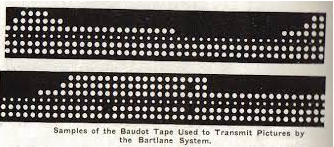
\includegraphics[width=0.8\textwidth]{imagenes/telegrafo}
\caption{Tira de Baudot.}
\label{telegrafo}
\end{figure}

\begin{figure}[h]
\centering
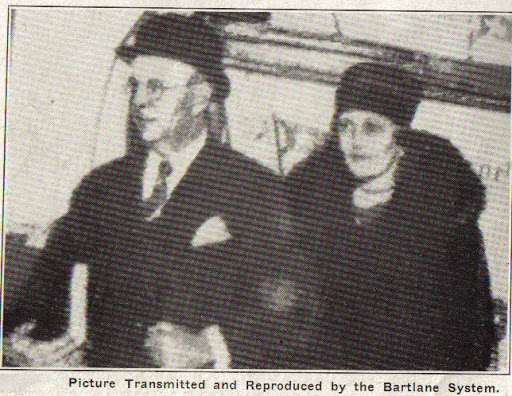
\includegraphics[width=0.8\textwidth]{imagenes/1digital}
\caption{Imagen transmitida usando el sistema de Bartlane.}
\label{1digital}
\end{figure}

Los avances en este campo en los primeros años dependían completamente del avance de los ordenadores y su capacidad tanto de almacenamiento como computacional.\\

Los primeros avances en el tratamiento digital de imágenes se dieron en los años 70 en el campo de la medicina y en astronomía. En medicina lo que impulsó esta necesidad para analizar imágenes digitales fué la invención del TAC (tomografía axial computarizada) que consiste en una serie de algoritmos que toman varias fotografías realizadas con rayos x para construir una imagen tridimensional. Se usan varias operaciones de tratamiento de imagen para mejorar el contraste de la imagen o pasar los diferentes niveles de gris a color para facilitar la interpretación.\\

Una de las razones principales que hacen que este campo sea tan complejo es la diferencia en cómo vemos imágenes nosotros y cómo las ``ve'' un ordenador. Nuestro cerebro analiza imágenes siempre en un contexto y conreferencias para comparar, mientras que un ordenador recibe una serie de datos finitos en los que se ha perdido por el camino mucha información, por ejemplo si el objeto de la imagen es tridimensional, de dónde viene la imagen y el contexto de esa imagen. Esto hace que cosas que para la vista humana son obvias para un ordenador sean operaciones muy complejas que requieran múltiples transformaciones y algoritmos para extraer ciertas características que se puedan contrastar con una base de datos.\\

El tratamiento de imagen se puede dividir en 3 procesos diferentes que se pueden dar secuencialmente en el análisis de una imagen o a la vez. Estos procesos son: pre-procesado, segmentación y análisis. La asignatura de TDI se centra sobre todo en métodos de pre-procesado y segmentación de imágenes.\\ 

\subsection{Aplicaciones}
El tratamiento digital de imagen tiene aplicaciones en una amplia variedad de campos desde medicina a diseño, pasando por astronomía y robótica.  Estos son algunos ejemplos de campos en los que se usan herramientas de tratamiento de imagen:
\begin{itemize}
\item \textbf{Medicina y biología}: El tratamiento de imágenes digital se usa para una gran cantidad de análisis. Un ejemplo serían las imágenes médicas que es el proceso de crear una representación visual de la estructura interior de un cuerpo antes de una intervención. También crea una representación visual de cómo funcionan varios órganos o tejidos. Esto se consigue gracias a varios avances en métodos como las tomografías computarizadas o las resonancias magnéticas.\\

También dentro del campo de la biología el tratamiento de imagen se está empleando para analizar imágenes sacadas de microscopio por ejemplo para automatizar el cómputo de células en una imagen.\\

\item \textbf{Visión artificial y robótica}: Este campo consiste en intentar emular la visión humana usando el tratamiento de imagen. Su objetivo es reconocer objetos e información relevante de una forma similar a como lo hacemos los humanos. Se está aplicando sobre todo en el campo de la robótica, por ejemplo para casos como la conducción automática de los coches o robots.\\

\item \textbf{Restauración}: Otro campo en el que se usan las herramientas de tratamiento de imágenes es en la restauración de imágenes (figura \ref{restauracion} o videos dañados, ya sea por antigüedad o cualquier otra causa. \\

\begin{figure}[h]
\centering
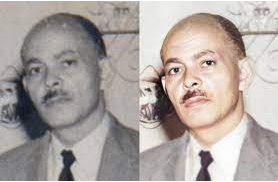
\includegraphics[width=0.8\textwidth]{imagenes/restauracion}
\caption{Imagen restaurada y coloreada usando tratamiento de imagen.}
\label{restauracion}
\end{figure}

\item \textbf{Geografía}: El tratamiento de imagen también se usa para crear mapas analizando imágenes de satélite y otros muchos análisis del terreno. Por ejemplo en agricultura Artizzu et al.\footnote{X. P. B. Artizzu, A. Ribeiro, A. Tellaeche, G.Pajares, C. F. Quintanilla (2009), Improving weed pressure assessment using digital images from an experience-based reasoning approach, Computers and Electronics in Agriculture, 65, pp. 176–185,
2009} diseñó un sistema que analiza imágenes del suelo y utiliza el color y la textura de la imagen para averiguar qué está plantado en esa zona.\\

\item \textbf{Seguridad}: Un tema por el que el tratamiento de imagen está recientemente en la noticias es su uso en seguridad, específicamente por la identificación facial en cámaras de seguridad. Este no es el único caso en el que se usa el tratamiento de imagen para seguridad, también se emplea en otras verificaciones biométricas, por ejemplo las huellas dactilares.\\

Otro ámbito de la seguridad en el que se usa el tratamiento de imagen es en la estenografía y la encriptación, por ejemplo para crear firmas digitales irremovibles en obras de arte o documentos.\\

\item \textbf{Transmisión y codificación}: Herramientas de tratamiento de imagen como el análisis de imágenes en frecuencia o  la reducción de niveles se usan amenudo para la codificación de imágenes y videos con el objetivo de que ocupen menos espacio y facilitar su transmisión.\\

\item \textbf{Diseño}: Por último mencionar el que seguramente sea el uso más común del tratamiento de imagen que es el diseño. Cualquier programa de uso común, como puede ser Photoshop, lo que tiene detrás de su interfaz son herramientas de tratamiento como filtros Gaussianos o filtros de detección de ejes.\\

\end{itemize}

\section{Educación accesible}

El tema principal de este proyecto es la educación como algo que debería ser gratuito y accesible al mayor número de personas posible

\section{La importancia de conocer las bases}

La razón por la que escogí 


\chapter{Objetivos}

\section{Objetivos}

El objetivo principal de este trabajo es crear una versión de las prácticas de la asignatura de Tratamiento Digital de la Imagen en Python. La asignatura se imparte en 3º de Ingeniería de sistemas audiovisuales y multimedia en la URJC y originalmente sus prácticas requieren el uso de Matlab. \\

El problema de utilizar Matlab surge de la necesidad de una licencia. Antes de la crisis de Covid-19 la URJC sólo pagaba licencia de Matlab para ordenadores que se encontrasen dentro del campus, esto crea un problema a la hora de consultar las prácticas cuando se está repasando para un examen o si se quieren probar diferentes partes de la teoría, sobre todo para alumnos que viven lejos del campus y no tienen vehículo propio.\\

Las nuevas prácticas se plantearon para funcionar en la plataforma de Robotics Academy. Por ello surgieron nuevos subobjetivos alrededor de la idea de que los ejercicios los pudiera realizar alguien que no está matriculado en la asignatura y por lo tanto no ha recibido las clases de teoría que acompañan las prácticas. El objetivo principal lo hemos articulado en tres subojetivos:
\begin{enumerate}
    \item Migrar las prácticas a cuadernillos de Jupyter
    \item Ampliar enunciados y explicaciones teóricas: Para que las prácticas se entiendan sin ir a clase de teoría se propone ampliar los enunciados con definiciones de conceptos básicos y enlaces a más recursos donde se explica en mayor profundidad cualquier elemento teórico.
    \item Prácticas en inglés: La plataforma de Robotics Academy está abierta para alumnos internacionales por lo que uno de los objetivos que se propuso fue traducir los enunciados de las prácticas al inglés.
\end{enumerate}

Por último y, con la misma idea de mejor accesibilidad, las nuevas prácticas deben ser multiplataforma, es decir, funcionar de la misma manera independientemente del sistema operativo que está usando el estudiante.

\section{Requisitos}

Para la realización del trabajo se imponen una serie de requisitos:
\begin{itemize}
    \item Se tiene que mantener la intención original de las prácticas, es decir, cambiar lo menos posible con el objetivo de demostrar la misma teoría que en la práctica original.
    \item Debe funcionar en diferentes sistemas operativos por lo que se probará todo tanto en Windows como en Ubuntu.
    \item Los enunciados deben ser fáciles de entender, con una gramática y estructura sencillas que no compliquen de manera innecesaria una asignatura ya de por sí compleja.
    \item Se evitarán ventanas emergentes, todo tiene que ser visible en el propio cuadernillo, de manera que una vez realizado sea fácil de consultar.
\end{itemize}

\section{Metodología}

En cuanto a la forma de llevar a cabo el trabajo se dividió el proceso de realizar las prácticas en una serie de pasos con un orden marcado. Además se mantuvieron tutorías semanales para ir comentando los avances y dudas que fueran surgiendo.\\

Las prácticas en general se fueron realizando en el mismo orden que se sigue en la asignatura. A medida que se avanzaba en el proyecto se fue desarrollando un método para optimizar el desarrollo de los ejercicios que consta de los siguientes pasos:

\begin{enumerate}
    \item Primero se vuelve a leer el enunciado de la práctica original en Matlab para refamiliarizarse con el tema que se trata.
    \item Se repasa la teoría para asegurar que se domina el tema. También se aprovecha este punto para ir recopilando posibles fuentes que se puedan poner de referencia en el enunciado final.
    \item Hacer la práctica en Matlab e ir haciendo capturas de los resultados que deben salir, tanto para comparar como para usar en esta memoria.
    \item Crear el cuadernillo de Jupyter. Se copia el enunciado original en español y se va subdividiendo en tareas que se puedan realizar en una celda de código sin ser abrumadoras.
    \item Comprobar las imágenes usadas en el ejercicio. Algunas de las imágenes que se usan en las prácticas de TDI no son de libre uso, para poder subir las prácticas a una plataforma como Robotics Academy o simplemente Github es mejor asegurarse de que las imágenes se puedan usar legalmente, sin problemas de propiedad intelectual.
    \item En caso de que alguna de las imágenes no sea de libre uso buscar alternativas que sirvan para demostrar lo mismo que mostraban las imágenes originales.
    \item Empezar a programar. Esto consiste en ir haciendo la práctica en Python buscando funciones en diferentes librerías de Python que funcionen lo más parecido posible a las de Matlab. En este punto se pueden dar tres situaciones diferentes:
        \begin{itemize}
            \item Que se encuentre una función con un funcionamiento exacto a la de Matlab. Este es el caso ideal.
            \item Que se encuentren una o más funciones cuyo resultado sea similar al de Matlab pero no exacto. En el caso de que sólo se encuentre una se investiga a qué se deben las diferencias y si se puede modificar el funcionamiento de la función con diferentes parámetros para que de un resultado lo más parecido posible. En caso de que se encuentre más de una función pero ninguna exacta se cogerá la más parecida.
            \item  No existe ninguna función equivalente en Python
        \end{itemize}
    \item Si se da el segundo caso del punto anterior se pasa a evaluar la diferencias, si son muy pequeñas se usa la función de Python teniendo en cuenta las pequeñas diferencias en el resto de la práctica y se va modificando acorde a la nueva imagen. Si las diferencias son muy grandes o no existe función se pasa a programar una nueva función en Python que sí cumpla los requisitos necesarios.
    \item A continuación se ejecuta la práctica entera comprobando los resultados con las capturas de Matlab del principio. Si no son satisfactorios se modifica el código donde sea necesario.
    \item Una vez el código da buenos resultados se procede a empezar la traducción/redacción del enunciado.
    \item Terminada una primera versión del nuevo enunciado se hace una revisión añadiendo los enlaces a fuentes y expandiendo información donde sea necesario.
    \item El último paso consiste en crear las celdas de respuesta con imágenes del aspecto que tendría que tener el resultado de la práctica para guiar a los alumnos.
    \item Antes de dar por completada la práctica se hace un último repaso del enunciado comprobando que no hay errores gramaticales y se crea una versión nueva en la que las celdas de código están vacías. Esta es la versión que se le dará al alumno.
\end{enumerate}

A grandes rasgos se han ido siguiendo estos pasos en todos los ejercicios. En caso de que surgiera una duda ya más de criterio que pudiese afectar al desarrollo de la práctica y desviarla de la original se consulta con Inmaculada Mora, la profesora que creó las prácticas, para asegurar que se mantiene la intención original y que los resultados son correctos.
\chapter{Infraestructura}

En esta sección se detallan tanto el software empleado para la realización del trabajo, como la estructura previa que existía en la asignatura y que ha servido como base para las nuevas prácticas. \\

 El lenguaje de programación utilizado ha sido Python. Profundizaremos en las bibliotecas que tiene este lenguaje para el tratamiento de imagen que han sido necesarias para el desarrollo del trabajo. Esta sección también explicará en que consiste la plataforma Jupyter Notebook y las ventajas que tiene en su uso para la docencia. Por último, se hablará de Matlab, la plataforma original que se usa en la asignatura de Tratamiento Digital de la Imagen y la estructura general que tienen las prácticas de esta asignatura.

\section{Python tratamiento de imagen y visualización}

Python\footnote{https://www.python.org/} es un lenguaje de programación interpretado de alto nivel orientado a objetos, creado en los años 80 por Guido van Rossum. Se caracteriza por tener una sintaxis sencilla, fácil de leer, lo que facilita el mantenimiento de programas y lo hace accesible para principiantes. Tiene una amplia biblioteca base y además permite el uso de módulos y paquetes. Al ser interpretado en lugar de compilado el proceso de depuración es más rápido. En este trabajo se ha usado la versión 3.7.4 de Python.\\

 Python se está usando cada día más para el tratamiento de imagen, esto se debe a que es un lenguaje muy accesible, siendo gratuito y con una sintaxis sencilla. Con el tiempo han ido surgiendo bibliotecas específicas para el tratamiento de la imagen en Python como Pil (Python Imaging Library) también llamada Pillow, Scikit-image y Open-CV. Esta última será la que más se use en este proyecto.\\

Otra biblioteca que facilita el tratamiento de imagen en Python es Numpy, una biblioteca para facilitar el uso de matrices y arrays en Python, así como las funciones matemáticas relacionadas.  Además, Matplotlib permite  la representación de datos en forma de gráficos.

\subsection{OpenCV}

OpenCV (Open Source Computer Vision Library)\footnote{https://opencv.org/} es una biblioteca centrada en el tratamiento de imagen y video (Computer Vision) y en aprendizaje de máquina, con interfaces para varios lenguajes de programación como C++, Python o Java. OpenCV es la biblioteca de procesamiento de imagen más usada en el mundo con más de 18 millones de descargas. Originalmente programada en C; el resto de lenguajes usa diferentes interfaces para acceder al código. Esto permite tener un buen rendimiento por ser C un lenguaje muy rápido en ejecución.\\

OpenCV contiene desde funciones de bajo nivel para el procesado de imagen hasta algoritmos complejos para deteccion de caras. En este trabajo, ya que trata de dar una base de tratamiento de imagen, usaremos funciones de bajo nivel como filtros o funciones para cambiar de espacio de color.\\

Se ha usado la versión 4.2.0 de OpenCV.\\


\subsection{Numpy}

Numpy\footnote{https://numpy.org/} es el paquete principal para cálculos complejos con matrices en Python, esto lo convierte en un paquete esencial en el desarrollo de código para usos ciéntificos y de robótica. La base de esta biblioteca es el objeto \emph{ndarray}, que consiste en arrays de n-dimensiones con datos de un mismo tipo y un tamaño establecido al crear la variable, esto último lo diferencia de las listas de Python que son dinámicas.\\

En este trabajo se ha usado la versión 1.16.5 de Numpy.\\

Numpy contiene funciones que permiten realizar operaciones con grandes cantidades de datos de una forma más eficiente en memoria y rápida que usando las funciones propias de Python. Numpy está programado y pre-compilado en C. El uso de las funciones de Numpy también permite que el código se parezca más a la notación matématica estándar, lo que lo hace más fácil de leer y entender.\\

\subsection{Matplotlib}

Matplotlib\footnote{https://matplotlib.org/} es una biblioteca para la creación de gráficos en Python. También permite la representacion de imágenes. Matplotlib está construido usando Numpy para funcionar con el paquete general de Scipy. Permite interactúar con los gráficos de una forma muy similar a la representación de Matlab. Matplotlib funciona sobre cualquier sistema operativo. \\

Una de las razones por las que se ha elegido esta biblioteca para representar las diferentes imágenes y gráficos de las prácticas de TDI es por cómo interactúa con los cuadernillos de Jupyter, ya que permite la visualización de los gráficos incrustrada en el propio cuadernillo sin crear otra ventana. \\

Otro punto a favor de Matplotlib es la capacidad para interactuar con los gráficos, cómo ya se ha mencionado antes, esto es algo que permite Matlab e interesaba mantener en las prácticas, ya que puede ayudar mucho a la hora de entender algunos de los ejercicios. Esta interactividad consiste en la posibilidad de hacer zoom en los gráficos y un cursor que indica el valor del pixel sobre el que está.\\

Se ha usado la versión 3.1.1.\\

\subsection{Scikits}

Abreviatura de Scipy Toolkits\footnote{https://www.scipy.org/scikits.html} son una serie de paquetes añadidos para Scipy separados de su distribución principal. Estos paquetes se separan de Scipy cuando se consideran demasiado específicos para el propio Scipy, por una licencia incompatible con la de Scipy o si aún están en desarrollo.\\

En este trabajo se van a usar 2 de esos kits:\\


\begin{itemize}

	\item \textbf{Scikit-learn}\footnote{https://scikit-learn.org/stable/}: Es un paquete con un amplio rango de algoritmos de aprendizaje de máquina para problemas de tamaño medio, tanto supervisados como no supervisados. Está programado mayoritariamente en Python aunque incorpora algunas bibliotecas de C++ e incorpora código compilado para mejorar su eficiencia.

	\item \textbf{Scikit-image}\footnote{https://scikit-image.org/}: Este paquete cuenta con una colección de algoritmos para el tratamiento de imagen construida por una comunidad de voluntarios.
\end{itemize}
\section{Cuadernillos de Jupyter}

El cuadernillo Jupyter\footnote{https://jupyter.org/} es una interfaz web de código libre, que permite la creación de documentos que contienen código ejecutable, ecuaciones, visualización (gráficos, imágenes) y texto.\\

El cuadernillo se guarda como un JSON la extensión \texttt{.ipnyb}. La aplicación es un modelo cliente-servidor que se ejecuta a través de un navegador. Se trata de un servidor local que se crea al ejecutar la aplicación lo que implica que no se necesita conexión a internet para leer o modificar un cuadernillo.  El servidor lee el documento \texttt{.ipnyb} y manda mensajes usando ZeroMQ (una librería que manda mensajes usando un modelo asíncrono) a un kernel que ejecuta el código Python en el cuadernillo. El cliente funciona en un navegador y es lo que permite interactuar con el cuadernillo, según se muestra en la Figura \ref{estructurajupyter}\\

\begin{figure}[h]
\centering
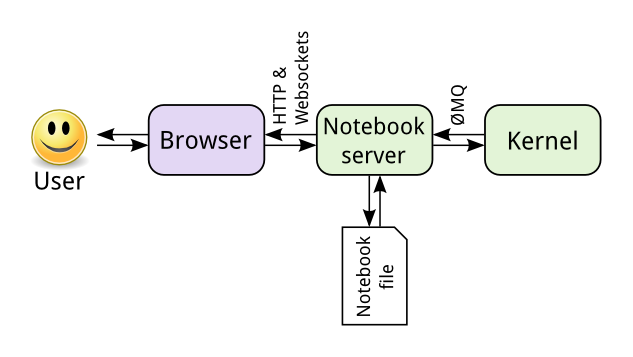
\includegraphics[width=1.0\textwidth]{imagenes/estructurajupyter}
\caption{Estructura de Jupyter Notebook.}
\label{estructurajupyter}
\end{figure}

Los cuadernillos de Jupyter consisten principalmente en dos tipos de celdas: \emph{code} y \emph{markdown}.\emph{ Code }son las celdas ejecutables en las que se escribe código de Python, mientras que \emph{markdown} son las celdas de texto. Para estilizar el texto se usa  la sintaxis de markdown, que permite desde poner texto en negrita hasta insertar imágenes o fórmulas matemáticas complejas.\\

En la Figura \ref{versionjupyter} se pueden ver las versiones de los diferentes paquetes necesarios para ejecutar un cuadernillo de Jupyter.

\begin{figure}[h]
\centering
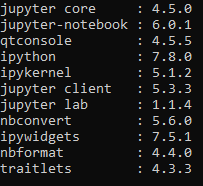
\includegraphics[width=0.5\textwidth]{imagenes/versionjupyter}
\caption{Imagen de una terminal que muestra las versiones de los paquetes de Jupyter usados en este trabajo.}
\label{versionjupyter}
\end{figure}


\section{Prácticas de TDI en Matlab}


Las prácticas originales para la asignatura de Tratamiento Digital de la Imagen consisten en una carpeta zip que se pone a disposición de los alumnos en el aula virtual de la asignatura. Dentro de esta carpeta están las imágenes que se van a utilizar en la práctica (cuando no eran imágenes internas de Matlab), funciones adicionales necesarias en caso de que no existieran previamente y un enunciado en pdf. En la Figura \ref{carpetapracticas} se puede ver un ejemplo de una de estas carpetas.\\
 
\begin{figure}[h]
\centering
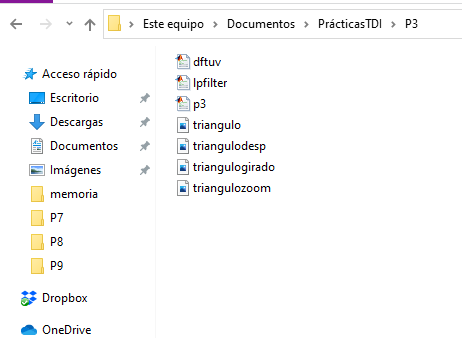
\includegraphics[width=0.5\textwidth]{imagenes/carpetapracticas}
\caption{Ejemplo de carpeta de prácticas.}
\label{carpetapracticas}
\end{figure}

Las prácticas se realizaban en hora de clase en uno de los laboratorios de Windows del campus. Se podían realizar enteras en la duración de la clase. \\

La profesora daba una breve explicación inicial sobre el tema de la práctica, siempre relacionado con lo que se hubiera dado en las clases de teoría recientes. El resto de la práctica se podía seguir de forma libre con el enunciado, con la profesora respondiendo las dudas que surgieran en el desarrollo del ejercicio. \\

Los enunciados son instrucciones detalladas sobre los pasos a seguir para realizar la práctica, con poco o nada de teoría, ya que se asume que el alumno ha recibido las clases de teoría previas. El alumno debe crear un nuevo documento en Matlab e ir ejecutando paso a paso lo que pide el enunciado. \\

Los enunciados suelen comenzar con un breve párrafo explicando el objetivo de la práctica. Por ejemplo en la práctica 4 que trata el tema de segmentación de imagen, la introducción dice:\emph{``El objetivo de esta práctica es comenzar a familiarizar al alumno con las herramientas básicas de segmentación de imagen en entorno MATLAB. Para ello se trabajará con la imagen en escala de
grises ‘calculadora.tif’, que acompaña al material de esta práctica. "}\\

A partir de esta breve introducción la práctica suele estar dividida en secciones normalmente relacionadas con diferentes puntos tratados en la teoría y cómo llevarlos a cabo.\\

Los pasos a seguir en Matlab, por lo general, vienen dados en el enunciado que indica qué función usar y cómo llamar a las diferentes variables para mantener una consistencia en los nombres a lo largo de la práctica. En algunos casos se indican las variables necesarias para llamar a la función que se va a usar en esa sección del ejercicio, mientras que en otros se pide al alumno que use el comando \textsl{+help} para informarse sobre el funcionamiento de la función. Del mismo modo, si una función requiere de un valor a decidir, dependiendo de lo que se quiera conseguir con su uso, unas veces se da con el enunciado y otras se deja a criterio del alumno para que pruebe cómo cambian los resultados con diferentes variables y cuál sería la mejor solución para el problema planteado.\\

Otra característica común de los enunciados de TDI son las preguntas para responder, aunque no se pide una memoria en sí de las prácticas en los enunciados hay preguntas con el objetivo de que el alumno se plantee las respuestas y las razones de los pasos que se han ido realizando durante el ejercicio.  La Figura \ref{preguntasp4} muestra un ejemplo de estas preguntas del principio de la práctica 4.

\begin{figure}[h]
\centering
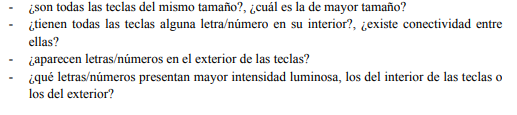
\includegraphics[width=1\textwidth]{imagenes/preguntasp4}
\caption{Ejemplo de preguntas realizadas en los enunciados de TDI.}
\label{preguntasp4}
\end{figure}

Algunos de los enunciados tienen imágenes del aspecto que tendría que tener la imagen sobre la que se está trabajando después de ciertos pasos para que el alumno pueda ver si el ejercicio progresa adecuadamente o si debería modificar alguna variable o revisar el código.\\

Si se pide un algoritmo un poco más complejo, en los enunciados aparece dado un trozo de ese código como ejemplo o directamente para copiar en Matlab ya que el objetivo de estas prácticas no era aprender a programar en Matlab sino ilustrar de forma práctica lo dado en teoría de la asignatura.\\

Las prácticas se suelen centrar en el tratamiento de una imagen en específico, elegida para ilustar el tema del que trata la práctica. Por ejemplo en la práctica 1, en el apartado que trata sobre color se escoge una imagen con diferentes verduras que muestran una variedad de colores para ilustrar la mezcla aditiva de color al representarse individualmente las matrices de cada color del sistema de representación RGB. Debido a que algunas de las imágenes usadas en las prácticas originales pertenecen a Matlab o se desconoce su origen se ha tenido que buscar imágenes nuevas, siempre intentando mantener las características de la imagen original.\\

En total la asignatura consiste de 9 prácticas, 7 de imagen y 2 de video. \\

\begin{itemize}
  \item [ P1.]\emph{Introducción al tratamiento de imagen:}\\
	Esta práctica es una introducción a las herramientas de tratamiento de imagen en Matlab. Se trata cómo leer y representar imágenes, espacios de color, escalado e histogramas. El último apartado se centra en imágenes RGB.
  \item [P2.]\emph{Filtrado de imágenes en el dominio espacial:}\\
	Esta práctica demuestra el funcionamiento de diferentes tipos de filtros sobre imágenes contaminadas con varios ruidos. En la segunda parte se tratan filtros de realce de contorno y se demuestra su uso para extraer los bordes de unas monedas.
  \item [P3.]\emph{Filtrado de imágenes en el dominio espectral:}\\
	En esta práctica se demuestran las propiedades de la transformada de Fourier y cómo afectan las transformaciones en el espacio a la representación en frecuencia de la imagen. También se tratan filtros en el dominio frecuencial.
  \item [P4.]\emph{Segmentación de imagen:}\\
	Esta práctica es diferente a las anteriores ya que en lugar de ejercicios individuales se centra en el tratamiento de una imagen en concreto con un objetivo claro. Se trata  la imagen de una calculadora con el objetivo de conseguir una nueva imagen en la que solo se vea la letra Enter de la calculadora. Para esto se usa segmentación binaria que es el tema de la asignatura que se corresponde con esta práctica.
  \item [P5.]\emph{Segmentación de imagen II:}\\
	Esta práctica sigue el esquema de la anterior centrándose en la segmentación de una imagen, en este caso un pájaro. Para la segmentación de este pájaro se va a usar aprendizaje de máquina, específicamente el algoritmo K-medias, la mayor parte de la práctica se centra en realizar diferentes transformaciones sobre la imagen para facilitar el uso del algoritmo. Entre estas transformaciones se encuentran cambios de espacio de color y filtros de textura.
  \item [P6.]\emph{Morfología binaria:}\\
	Este ejercicio aplica operaciones de morfología matemática para segmentar los chips de una placa y separarlos de acuerdo a su forma.
  \item [P7.]\emph{Segmentación por watershed:}\\
	El objetivo de esta práctica es segmentar una imagen con células para contarlas. Para conseguir esto se plantea el uso del algoritmo de \emph{watershed} con marcadores. Primero se extraen los marcadores internos de las células usando herramientas como la reconstrucción morfológica y conseguir los máximos regionales de una imagen, operaciones estudiadas en la parte correspondiente a esta práctica del temario. Lo mismo ocurre con los marcadores exteriores y el uso de la transformada de distancia. Esta práctica además tiene el objetivo de demostrar que la segmentación de este tipo de elementos que muchas veces se encuentran superpuestos en una imagen es muy complicada y siguen dando bastante error.
  \item [P8]\emph{Manejo de vídeos en Matlab. Detección y estimación de movimiento:}\\
	Esta es la primera de las prácticas de video, está dividida en dos secciones claras. La primera es una introducción a las herramientas de video en Matlab, estructura de video, como reproducir y guardar videos. La segunda trata 3 algoritmos de estimación de movimiento: EBMA, HBMA y correlación de fase.
  \item [P9]\emph{Mejora y restauración de vídeo. Filtrado interframe:}\\
	La segunda práctica de vídeo y la última de la asignatura trata la restauración de video contaminado con ruido de una forma muy similar a la práctica 2 de imagen. Primero se centra en el filtrado fotograma a fotograma y después en el filtrado \emph{interframe}, es decir usando varios fotogramas para compararlos entre si y así filtrar.
\end{itemize}


\chapter{Prácticas de TDI}

Este apartado trata el desarrollo y resultado del proyecto, se irá analizando cada práctica de la asignatura y comparando la versión original con el resultado final en Python. Se tratarán también los diferentes problemas que han ido surgiendo a la hora de adaptar cada práctica y cómo se han solucionado.\\

\section{Estructura de las prácticas en Jupyter Notebook}

A la hora de plantear las prácticas en los cuadernillos de Jupyter lo primero que se hizo fue decidir qué partes se iban a mantener igual y en qué se iban a diferenciar de las de Matlab. La estructura en si, el temario tratado, el orden de los ejercicios y en los casos que se podía las imagenes originales se intentan mantener intactas. Lo más importante era mantener el cometido de la práctica, lo que se pretendía mostrar y enseñar con ella.\\

El cambio más obvio entre las dos versiones de los ejercicios tiene que ver con los enunciados, en los cuadernillos el enunciado está en inglés ya que se planteó el TFG para subir las prácticas a Robotics Academy, esto las haría más accesibles a un mayor número de estudiantes internacionales, no sólo de la URJC. Otro cambio en los enunciados es que han sido ampliados, esto se debe a que las prácticas originales son un material que se apoya sobre la teoría dada en clase y asumen que esa teoría ha sido impartida, mientras que en Robotics Academy las prácticas serían el único contacto que tendría el alumno con el tema por lo que los nuevos enunciados amplían un poco las explicaciones teóricas añadiendo enlaces a más recursos para ampliar conocimientos.\\

Una cosa común en los enunciados originales son los trozos de código facilitados para copiar y pegar, en Jupyter estas líneas de código aparecen en celdas tipo \emph{code} con indicaciones para cambiar los nombres de las variables si es necesario.\\

En cuanto al desarrollo de los ejercicios el cambio principal es el lenguaje de programación, de Matlab a Python. \\

Un cambio significativo en la presentación de la práctica es el uso de ventanas emergentes. Cuando ejecutas las prácticas en Matlab con la cantidad de imágenes que se pide representar pueden aparecer hasta 20 pestañas nuevas  (Figura \ref{ventanas}) lo que puede ser bastante abrumador. En la versión desarrollada en este trabajo se han evitado las ventanas emergentes, representando siempre que se ha podido en el propio cuadernillo, esto también hace las prácticas más fáciles de consultar una vez se ha terminado el código ya que se puede guardar el cuadernillo una vez ejecutado y las imágenes se mantienen mientras no se vacíe el output.\\

\begin{figure}[h]
\centering
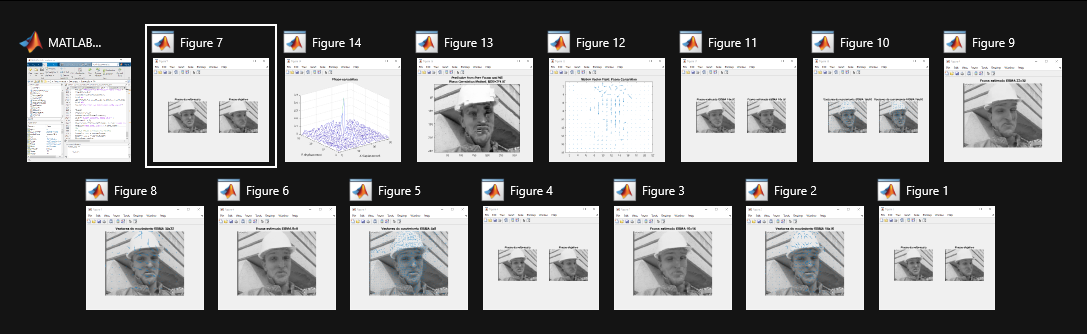
\includegraphics[width=1\textwidth]{imagenes/ventanas}
\caption{Ventanas emergentes en el apartado 2 de la práctica 8 en Matlab.}
\label{ventanas}
\end{figure}

Por último, en los cuadernillos se ha añadido un nuevo apartado donde se muestra el aspecto que tiene que tener la imagen resultante de algunos apartados de la práctica. En una clase práctica de TDI siempre estaba la profesora, esto permitía que en caso de duda se le pudiese preguntar si iba bien la práctica enseñando la imagen resultado de un apartado en el que se tuviera duda. Las imágenes respuesta pretenden sustituir esta opción para los alumnos que accedan a las prácticas fuera del contexto de la asignatura de TDI en la URJC.


\section{Guía de instalación}

Para facilitar el acceso a las prácticas se ha creado una guía de instalación en \emph{markdown} directamente accesible en Github desde el repositorio en el que están las prácticas.\\

La guía requiere que primero se compruebe si el ordenador tiene instalado Python3, en caso negativo, se pone un link a la página oficial de Python con la guía de instalación para los diferentes sistemas operativos.\\

A continuación, se indica cómo instalar Pip, el instalador de paquetes en Python y se indica el comando para instalar Pipenv.\\

La guía continúa explicando cómo acceder a la prácticas y como iniciar el entorno de Pipenv necesario para ejecutarlas.\\

Por último, se explica cómo abrir un cuadernillo de Jupyter importando las librerías necesarias en la primera práctica para comprobar que el entorno se ha instalado correctamente.\\

Esta guía está en inglés, al igual que las prácticas y pensada para ser usada y funcionar por igual en cualquiera de los principales sistemas operativos. Ha sido probada en Windows de Microsoft y Linux Ubuntu.\\

\section{Práctica 1: Introducción}

\subsection{Teoría tratada}

En esta práctica\footnote{\url{https://github.com/RoboticsLabURJC/2019-tfg-ana-cuevas/blob/master/PracticasTDI/P1/1_Introduction.ipynb}} se opera sobre la matriz de la imagen, también se explica de forma práctica la diferencia entre una imagen \emph{true color} y una imagen indexada. Se pone un énfasis especial en los diferentes tipos de datos en matrices (double, uint64, float...) ya que a la hora de operar puede dar lugar a error.\\

El segundo punto de la práctica se centra en la conversión de imágenes de color a gris y binario. A continuación se usan diferentes métodos para modificar la resolución de una imagen actuando tanto sobre la resolución espacial como sobre la intensidad.\\

La práctica también explica cómo representar el histograma de una imagen y el efecto que tiene la ecualización del histograma sobre el contraste de la imagen.\\

Por último se ve la interpretación del color y cómo realizar transformaciones puntuales.\\

\subsection{Comparativa Matlab vs Python}

En este apartado mencionamos las principales diferencias entre la práctica realizada en Matlab y el nuevo formato usando un cuadernillo de Jupyter.\\

En el primer apartado de la práctica, que se centra en la lectura y representación de imágenes, podemos encontrar dos diferencias:\\

\begin{itemize}
\item La primera es el espacio de color sobre el que se trabaja. Matlab y Matplotlib leen las imágenes de color como RGB mientras que OpenCV usa BGR, esto genera un conflicto entre la librería que se va a usar para leer imágenes y la que se va a usar para representar. Se resuelve en el siguiente apartado que trata sobre espacios de color.\\

\item La segunda son los métodos de representación. En Matlab teníamos una única funcion (\texttt{imshow}) que crea una ventana nueva con la imagen representada y herramientas como un cursor y la posibilidad de hacer zoom. En Pyhton tenemos dos opciones de representación, una es \texttt{imshow} en la biblioteca  OpenCv, que al igual que Matlab genera una ventana nueva fuera del cuadernillo pero no tiene herramientas, y la otra es \texttt{imshow} en Matplotlib que permite visualizar la imagen en el propio cuadernillo y tiene las mismas herramientas que Matlab.\\
\end{itemize}

La siguiente gran diferencia entre los dos ejercicios es en el apartado de conversión de tipos de imágenes. Como ya se mencionó, se ha añadido una transformación de espacios de color para solucionar el problema de lectura, pero la mayor diferencia tiene que ver con la falta de una función que convierta una imgen RGB a indexada que sí existe en Matlab. Se probó a programar una versión equivalente en Python pero por cuestión de velocidad en la ejecución no se pudo implementar. El problema se solventó exportando las dos matrices que forman una imagen indexada desde Matlab  e implementarlas en Python aprovechando para explicar cómo se crean los mapas de color.\\

La falta de la función \texttt{RGB2ind} vuelve a ser relevante en el punto sobre modificación de la resolución de intensidad de una imagen, ya que en la práctica original se usaba esta función para cambier el número de niveles de intensidad en el mapa de color. Se resuelve explicando una resolución matemática al problema sin cambiar la imagen a indexada. Al ser una imagen en escala de grises con menos información que una imagen RGB también se puede usar la versión de Python de \texttt{RGB2ind} ya que el tiempo de ejecución es menor para imágenes en escala de grises. En la figura \ref{resmatematica} se puede ver la parte del enunciado en la que se explica la resolución matemática. 

\begin{figure}[h]
\centering
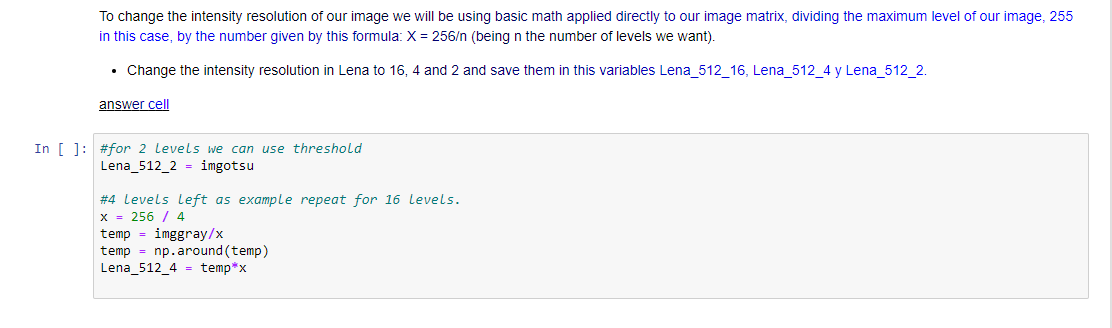
\includegraphics[width=1\textwidth]{imagenes/resolucionmatematica}
\caption{Enunciado del apartado sobre resolución de intensidad.}
\label{resmatematica}
\end{figure}

En el apartado sobre el histograma, el único cambio es la imagen utilizada para ejemplificar la ecualización del histograma, ya que la imagen original pertenece a Matlab. Sucede lo mismo en el último apartado con la imagen de los pimientos.\\

Por último, en los cuadernillos se ha añadido un nuevo apartado donde se muestra el aspecto que tiene que tener la imagen resultante de algunos apartados de la práctica.

\subsection{Desarrollo de funciones}

En esta práctica solamente fue necesario desarrollar una función nueva: \texttt{RGB2ind}\footnote{\url{https://github.com/RoboticsLabURJC/2019-tfg-ana-cuevas/blob/master/PracticasTDI/P1/rgb2ind.py}}. Esta función se usa para convertir una imagen \emph{true color} RGB en una imagen indexada con el número de niveles como parámetro. \\

A la hora del desarrollo se intentó buscar el código de la función original de Matlab, pero es de las funciones precompiladas en C y su código no es accesible. Se resolvió usando el algoritmo K-medias con un número de núcleos igual al número de niveles requeridos.\\

 La función final tiene un problema de tiempo de ejecución. Para un número pequeño de núcleos funciona bien, pero por ejemplo para los 256 requeridos en la práctica el tiempo de ejecución interrumpiría el desarrollo cómodo del ejercicio. Para mejorarla se podría probar a usar una versión pre-compilada de Python o programar la función en C e implementarla.\\

La figura \ref{rgb2ind} muestra cómo queda la solución para una imagen indexada de 5 niveles.

\begin{figure}[h]
\centering
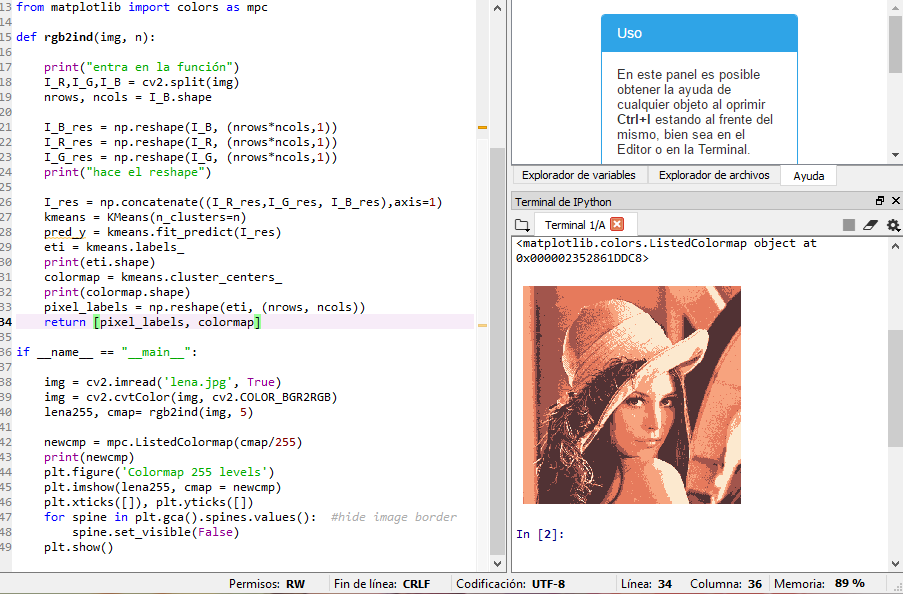
\includegraphics[width=1\textwidth]{imagenes/rgb2ind}
\caption{Muestra de código y solución de \texttt{RGB2ind}.}
\label{rgb2ind}
\end{figure}


\section{Práctica 2: Filtrado espacial}

\subsection{Teoría tratada}

Este segundo ejercicio\footnote{\url{https://github.com/RoboticsLabURJC/2019-tfg-ana-cuevas/blob/master/PracticasTDI/P2/2_Spatialfiltering.ipynb}} se centra en el filtrado de imágenes en el espacio, se irán demostrando diferentes tipos de filtro y sus usos más comunes en la práctica.\\

El primer apartado enseña diferentes tipos de ruido y cómo contaminar una imagen, los tipos de ruido tratados son: ruido gaussiano, ruido de sal y pimienta y ruido granular.\\

Los filtros se dividen en dos categorías: filtros paso bajo y filtros paso alto. En esta práctica se explican dos filtros paso bajos diferentes. El primero es el filtro de media que es un filtro lineal. Consiste en ir colocando una máscara sobre la imagen y calculando la media de los píxeles bajo la máscara, este filtro genera un suavizado de la imagen según se aprecia en la figura \ref{filtromedia}.

\begin{figure}[h]
\centering
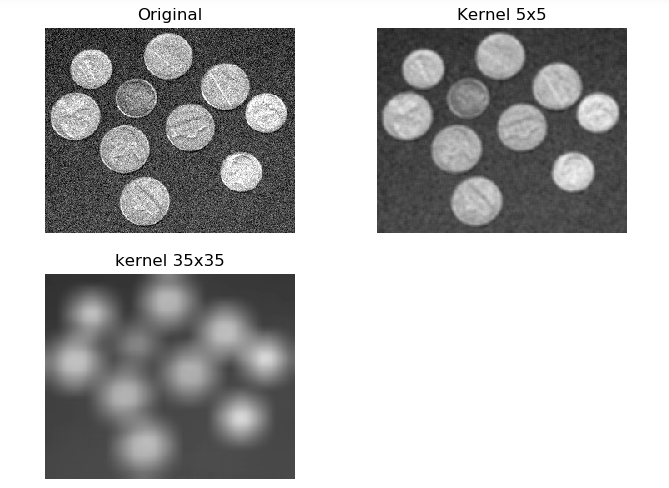
\includegraphics[width=1\textwidth]{imagenes/filtromedia}
\caption{Imagen del cuadernillo donde se demuestra el filtro de media con diferentes tamaños de máscara.}
\label{filtromedia}
\end{figure}

El otro filtro paso bajo es el filtro de mediana que es un filtro no lineal. Este filtro coge los valores de debajo de la máscara y  hace la mediana con esos valores, esto permite que se mantengan mejor los valores originales de la imagen, se usa para quitar ruido de sal y pimienta en la práctica.\\

Los filtros paso alto son filtros de realce de contornos. Se usan sobre todo para detectar bordes de objetos en la imagen. En esta práctica se dan dos tipos de filtro paso alto dependiendo de la máscara que usan: Prewitt e Isotrópico. Según se aprecia en la figura \ref{fpa}.

\begin{figure}[!tbp]
  \centering
  \subfloat[Prewitt.]{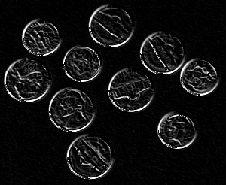
\includegraphics[width=0.4\textwidth]{imagenes/prewitt}\label{fig:f1}}
  \hfill
  \subfloat[Isotrópico.]{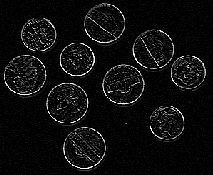
\includegraphics[width=0.4\textwidth]{imagenes/isotropic}\label{fig:f2}}
  \caption{Filtros paso alto.}
  \label{fpa}
\end{figure}

\subsection{Comparativa Matlab vs Python}

En el primer apartado de esta práctica se usan una serie de funciones que no pertenecen a Matlab y vienen entre los materiales de la práctica original. Estas funciones se recrean en Python con la misma funcionalidad.\\

En el apartado de filtros lineales la función más importante es \texttt{imfilter} que tiene de parámetros de entrada la imagen a filtrar, la máscara y el tipo de \emph{padding}. El tipo de \emph{padding} indica cómo se va a rellenar la máscara cuando el valor del centro es un borde de la imagen, los dos tipos de \emph{padding} que se demuestran en esta práctica son \emph{zero padding} que rellena con 0 y \emph{mirror padding} que copia los píxeles cercanos al borde. La función \texttt{filter2D} de OpenCv funciona de la misma manera y con los mismos parámetros.\\

Es importante mencionar que para apreciar bien las diferencias de tipo de \emph{padding} se tienen que ver bien los bordes de la imagen. Matplotlib, por defecto, añade un borde negro a sus figuras, esto impide que se aprecie bien la diferencia. Se encuentra un comando adicional para quitar estos bordes por defecto.\\

Para el filtro de mediana también existe una función en OpenCV \texttt{medianblur} que funciona exactamente igual que el equivalente de Matlab.\\

La mayor diferencia en el apartado de realce de contornos la encontramos en la función \texttt{fspecial} de Matlab que genera máscaras específicas para los diferentes filtros paso alto. Esta función no existe en OpenCV, se usa Numpy para generar las matrices y se van metiendo los valores correctos de acuerdo con el tipo de filtro que se quiere usar. Para hacer el filtrado en sí se usa la misma función que para los filtros lineales paso bajo.\\

El último apartado de composición de imágenes requiere funciones que se usaron ya en la práctica 1 y una función nueva de Numpy para realizar sumas punto a punto de matrices de más de dos dimensiones. La solución final queda muy parecida a la original de Matlab. Según se aprecia en la figura \ref {p2final}\\


\begin{figure}[!tbp]
  \centering
  \subfloat[Matlab]{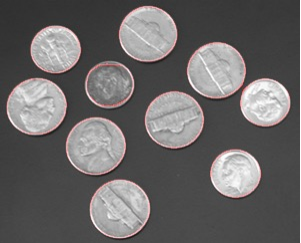
\includegraphics[width=0.4\textwidth]{imagenes/finp2ml}\label{fig:f1}}
  \hfill
  \subfloat[Python]{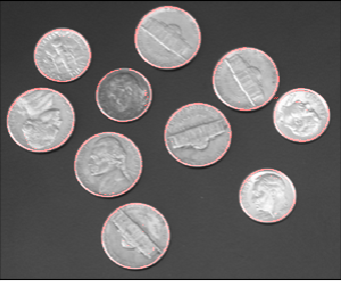
\includegraphics[width=0.4\textwidth]{imagenes/finp2py}\label{fig:f2}}
  \caption{Imágenes resultado del último apartado de la práctica 2.}
  \label{p2final}
\end{figure}


\subsection{Desarrollo de funciones}

Para este ejercicio se han tenido que desarrollar varias funciones, todas relacionadas con la función de añadir ruido en una imagen. Todas se encuentran en un único documento 'imfunctions.py'\footnote{\url{https://github.com/RoboticsLabURJC/2019-tfg-ana-cuevas/blob/master/PracticasTDI/P2/imfunctions.py}} que es importado al empezar la práctica. La función principal \texttt{imnoise} tiene 3 parámetros de entrada: la imagen a contaminar, el tipo de ruido y un parámetro genérico que indica los parámetros de cálculo del ruido (por ejemplo si el ruido es gaussiano este parámetro contiene la media y la varianza). La imagen puede ser tanto en tonos de gris como en color. Para añadir el ruido se llama a \texttt{addnoise} que es la función que realiza las operaciones matemáticas necesarias.\\

Otras funciones que se han ido creando por necesidad de \texttt{imnoise} son \texttt{checkcolor} que, como su nombre indica, se encarga de comprobar si la imagen es de color y un par de funciones para cambiar el tipo de datos de la matriz de imagen, por ejemplo, de \texttt{uint8} a \texttt{double} y viceversa.

\section{Práctica 3: Filtrado en el dominio de la frecuencia}
\subsection{Teoría tratada}

En esta práctica\footnote{\url{https://github.com/RoboticsLabURJC/2019-tfg-ana-cuevas/blob/master/PracticasTDI/P3/3_frequency.ipynb}} se trata la imagen en el dominio de la frecuencia. Se intenta mostrar de forma práctica cómo se ve una imagen en frecuencia y en qué consiste la transformada de Fourier bidimensional. Se explica porqué se necesitan dos representaciones diferentes para una misma imagen (módulo y fase) y qué representa cada una.\\

El segundo apartado demuestra las propiedades de la transformada de Fourier, qué transformaciones en el espacio afectan a la fase y cuáles al módulo y de qué manera.\\

El resto de la práctica se centra en el filtrado de imagen en el dominio frecuencial. Primero se explican dos filtros paso bajo: Gaussiano e ideal [Figura \ref {gauss}]. Se trata de filtrar la imagen en frecuencia y ver cómo afecta en el espacio tras hacer una tranformada de Fourier inversa.
\begin{figure}[h]
\centering
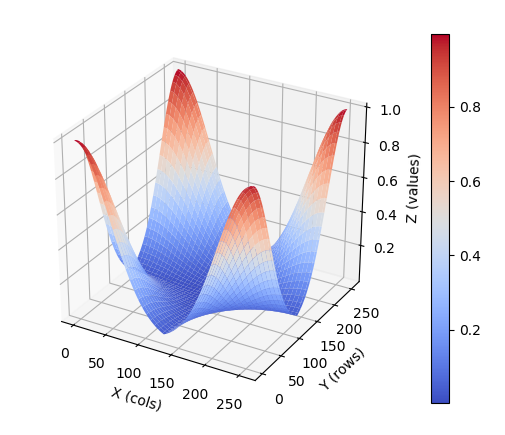
\includegraphics[width=0.6\textwidth]{imagenes/gaussfpb}
\caption{Representación gráfica de un filtro paso bajo Guassiano.}
\label{gauss}
\end{figure}

 Para concluir la práctica se tratan los filtros paso alto que, en el dominio de la frecuencia, son iguales que los filtros paso bajo pero invertidos.
\subsection{Comparativa Matlab vs Python}

En este ejercicio se usa una imagen dada con la práctica original de un triángulo blanco sobre un fondo negro.\\

La función más importante de esta práctica es \texttt{fft2}, la transformada de Fourier bidimensional. Existe un equivalente exacto en Numpy,  \texttt{numpy.fft.fft2}. También existe equivalente para la función \texttt{fftshift} que modifica la representación de la imagen en frecuencia para que las frecuencias bajas se concentren en el centro de la imagen y las altas en los extremos.\\

Para las representaciones en 3D se ha usado una función sacada de Github\footnote{\url{https://gist.github.com/CMCDragonkai/dd420c0800cba33142505eff5a7d2589
}} de código abierto que simplifica el código de forma que, para representar un gráfico, solo tienes que llamar a una función en lugar de meter todas las especificaciones de Matplotlib cada vez que se quiera representar algo. En el cuadernillo se deja el código demostrando cómo usar esta función.\\

El apartado de propiedades de la transformada de Fourier se mantiene igual de Matlab a Python. Como se ve en la Figura \ref{zoom}\\.

\begin{figure}[!tbp]
  \centering
  \subfloat[Matlab]{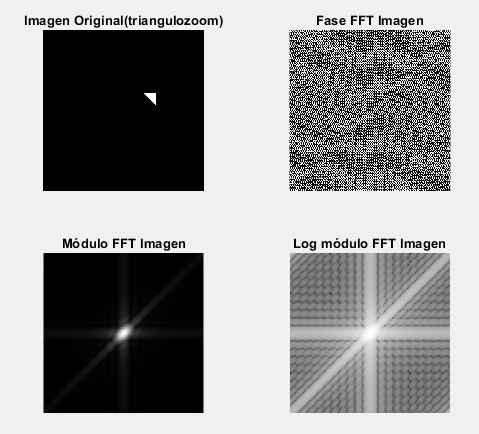
\includegraphics[width=0.5\textwidth]{imagenes/propml}\label{fig:f1}}
  \hfill
  \subfloat[Python]{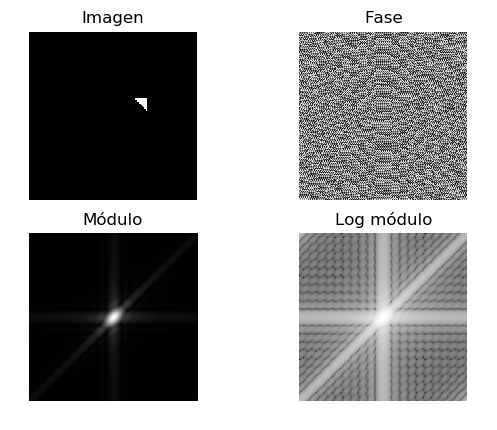
\includegraphics[width=0.5\textwidth]{imagenes/proppy}\label{fig:f2}}
  \caption{Comparativa de resultado en el apartado de propiedades de la transformada.}
  \label{zoom}
\end{figure}

Al igual que en la práctica anterior hay una función que viene dada con los materiales de la práctica, en este caso es  \texttt{lpfilter}, una función para generar filtros de tipo Guassiano o ideal. Se recrea con el mismo funcionamiento en Python. A la hora de filtrar, lo que en el espacio era una convolución (ir moviendo una máscara sobre cada pixel) en la frecuencia es una multiplicación punto a punto que se puede realizar con \texttt{numpy.multiply}.\\

El último apartado de filtros paso alto vuelve a usar la función \textbf{lpfilter} para después invertir el filtro de modo que actúe como un filtro paso alto. Para filtrar se repite el mismo proceso, como muestra la Figura \ref{fpa}].

\begin{figure}[h]
\centering
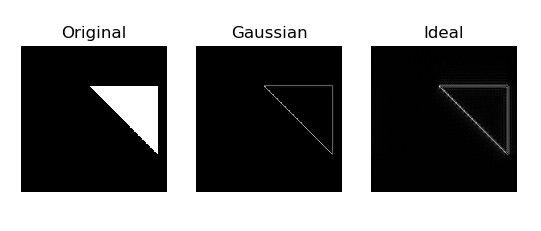
\includegraphics[width=0.7\textwidth]{imagenes/fpa}
\caption{Resultados del apartado sobre filtros paso alto.}
\label{fpa}
\end{figure}

\subsection{Desarrollo de funciones}

En esta práctica se ha desarrollado una función \texttt{lpfilter}\footnote{\url{https://github.com/RoboticsLabURJC/2019-tfg-ana-cuevas/blob/master/PracticasTDI/P3/lpfilter.py}} que, como se ha mencionado en el apartado anterior, genera filtros en frecuencia de dos tipos: Gaussiano e ideal. Como parámetros de entrada recibe el tipo de filtro que se quiere, las medidas del filtro que tienen que coincidir con las de la imagen que se quiere filtrar y D0 que es la apertura del filtro.\\

\section{Práctica 4: Segmentación de imagen I}
\subsection{Teoría tratada}

Esta práctica\footnote{\url{https://github.com/RoboticsLabURJC/2019-tfg-ana-cuevas/blob/master/PracticasTDI/P4/4_Segmentation.ipynb}} se centra en entender algunos métodos de segmentación de imágenes usando el ejemplo de una calculadora. En el proceso de segmentar una de las teclas de esta calculadora se van usando varios métodos dados en la teoría de la asignatura.\\

El primero de estos métodos es umbralización usando el histograma, que consiste en elegir un valor como umbral a la hora de convertir una imagen en binaria de forma que queden en primer plano las partes de la imagen que nos interesan. En este caso, las letras de la calculadora [Figura \ref{thresholding}].\\

\begin{figure}[h]
\centering
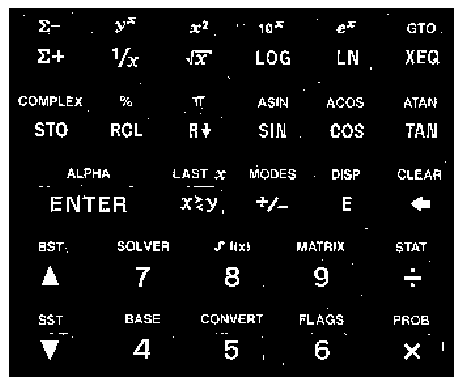
\includegraphics[width=0.6\textwidth]{imagenes/thresholding}
\caption{Imagen tras realizar la umbralización.}
\label{thresholding}
\end{figure}
A continuación se explican la segmentación y caracterización de regiones. Segmentación consiste en dividir la imagen en diferentes conjuntos de píxeles llamados regiones, esas regiones forman la capa de segmentación. A cada una de estas regiones se le asigna una etiqueta, la etiqueta 0 se le suele asignar al fondo.\\

Hay varios tipos de segmentación, en este caso se va a usar segmentación binaria que busca grupos conexos de píxeles de primer plano y asigna etiquetas. No todas las regiones van a ser de interés, ya que en muchos casos la umbralización inicial puede no ser perfecta, por ejemplo, por ruido. Para decidir qué regiones son de interés se pueden mirar diferentes características como pueden ser la forma o el tamaño. En este caso se usa el área de la región para decidir cuáles son de interés. Tras un proceso de filtrado la imagen queda como se puede ver en la Figura \ref{filtersmallareas}.\\


\begin{figure}[h]
\centering
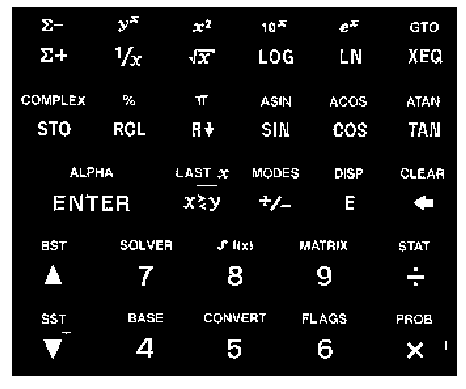
\includegraphics[width=0.6\textwidth]{imagenes/filtersmallareas}
\caption{Resultado de filtrar regiones de área pequeña.}
\label{filtersmallareas}
\end{figure}

En este punto, cada letra es una región propia pero lo que nos interesa segmentar son teclas. Se observa que la distancia entre letras de la misma tecla es muy inferior a la distancia entre letras en diferentes teclas. Para fundir las letras se usa un filtro paso bajo de media. Con esta nueva imagen se repiten todos los procedimientos anteriores hasta que se consigue segmentar solamente la tecla ENTER, tal y como se muestra en la  Figura \ref{finp4}.

\begin{figure}[h]
\centering

\includegraphics[width=0.6\textwidth]{imagenes/finp4}
\caption{Resultado final de la práctica 4 en Python.}
\label{finp4}
\end{figure}


\subsection{Comparativa Matlab vs Python}

En esta práctica hay muy pocas diferencias de Matlab a Python. El apartado de umbralización se mantiene igual, usando las funciones para el histograma y la umbralización que se utilizaron en la práctica 1.\\

En el apartado de segmentación en Python nos encontramos con dos opciones: la función de segmentación de OpenCV y la de la librería Scikit-image. Se usa la de Scikit-image ya que funciona de manera mucho más similar a la de Matlab, sobre todo a la hora de conseguir las propiedades de las etiquetas. En OpenCV la función que devuelve propiedades de etiquetas es muy limitada con muy poca información, mientras que la de Scikit-image devuelve casi exactas las mismas propiedades que el equivalente en MatLab.\\


 Se usan dos funciones para la segmentación y la caracterización de regiones. La primera es \texttt{bwlabel} en Matlab, \texttt{bwlabel} en scikit,  que crea las regiones con píxeles vecinos y devuelve una matriz del tamaño de la imagen original en la que a cada píxel se le ha asignado un número de acuerdo a su región, esta matriz es la capa de etiquetas. La segunda función es \texttt{regionprops}, se mantiene el mismo nombre en ambas versiones, que recibe de entrada la capa de etiquetas y devuelve medidas de algunas características de la capa de etiquetas, por ejemplo el área de cada región, la excentricidad o la posicion de los píxeles extremos de cada región.\\

La mayor diferencia entre label en Matlab y Scikit-image es el tratamiento de los píxeles de fondo. Matlab trata todo pixel de intensidad 0 como una única etiqueta de valor 0, mientras que Scikit-image, aunque en la imagen etiquetada pone los píxeles negros con la etiqueta 0, no lo cuenta como una etiqueta, por lo que, por ejemplo, en \texttt{regionprops} no tenemos la opción de recibir datos sobre los píxeles de fondo. A la función se le puede indicar que etiquete los píxeles negros pero no funciona igual que Matlab, ya que los trata como una etiqueta más, es decir, cuenta como etiquetas diferentes los píxeles negros no conexos. Esto no supone ningún problema en la realización de esta práctica excepto una ligera incomodidad ya que en el array devuelto por \texttt{regionprops} no coinciden los índices con el número de etiqueta en la imagen etiquetada, hay que sumarle uno al índice.\\

Para representar la capa de etiquetas en color Matlab tiene una función dedicada, mientras que en Python se puede usar cualquiera de los mapas de color disponibles de Matplotlib que generan el mismo efecto. En este caso se usa \emph{'nipy-special'} porque mantiene el fondo de color negro, tal y como se aprecia en la Figura \ref{color}.\\

El resto de la práctica usa la función de filtrado de media de la práctica 2 y repite los mismos pasos de los apartados anteriores.

\begin{figure}[h]
\centering
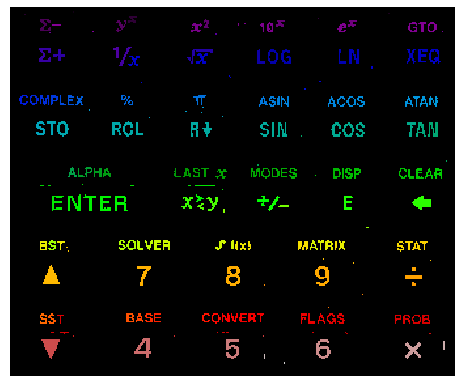
\includegraphics[width=0.6\textwidth]{imagenes/color}
\caption{Capa de etiquetas representada usando \emph{'nipy-special'}.}
\label{color}
\end{figure}


\section{Práctica 5: Segmentación de imagen II}
\subsection{Teoría tratada}

Esta práctica\footnote{\url{https://github.com/RoboticsLabURJC/2019-tfg-ana-cuevas/blob/master/PracticasTDI/P5/5_Segmentation2.ipynb}} continúa el tema de la práctica anterior. Intenta segmentar una imagen, en este caso es la figura de un pájaro que se puede ver en la Figura \ref{cormoran}. Para realizar este proceso de segmentación se va a usar aprendizaje de máquina K-medias.\\
\begin{figure}[h]
\centering
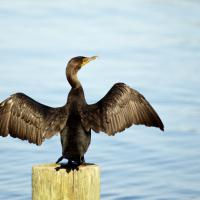
\includegraphics[width=0.6\textwidth]{imagenes/cormoran_rgb}
\caption{Imagen utilizada en la práctica 5.}
\label{cormoran}
\end{figure}

Usa un sistema de ensayo/error con el objetivo de que el alumno entienda que no todos los métodos funcionan igual para todas las imágenes porque cada imagen tiene unas características diferentes.\\

El primer método que se intenta para segmentar la imagen es el utilizado en la práctica anterior: umbralización. Al ver el histograma de la imagen del cormorán queda claro que la umbralización no va a ser posible, ya que no hay una distinción tan clara de tonos como en la imagen de la calculadora.\\

El siguiente método que se usa es el algoritmo K-medias aplicado sobre la imagen en RGB. Cogemos una descripción sencilla del funcionamiento de K-medias de la universidad de Oviedo: "K-means es un algoritmo de clasificación no supervisada (\emph{clusterización}) que agrupa objetos en k grupos basándose en sus características. El agrupamiento se realiza minimizando la suma de distancias entre cada objeto y el centroide de su grupo o cluster. Se suele usar la distancia cuadrática."\\

La característica sobre la que vamos a agrupar estos datos es el color, en este caso, se ordenan en una gráfica 3D donde cada eje es una componente de color en RGB (Figura \ref{cormoranrgb}).\\

\begin{figure}[h]
\centering
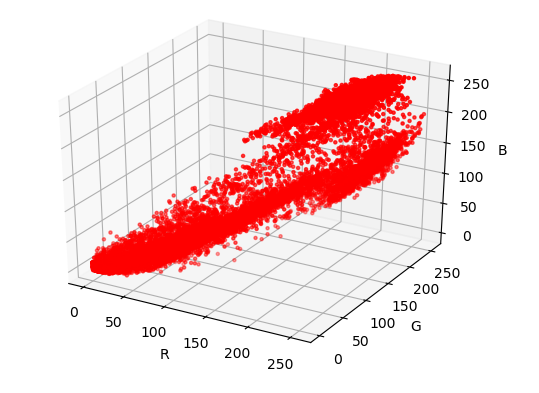
\includegraphics[width=0.6\textwidth]{imagenes/cormoranrgb}
\caption{Representación de los píxeles de la imagen en gráfico 3D.}
\label{cormoranrgb}
\end{figure}

 Se decide usar 3 centroides, ya que son los colores principales que se aprecian en la imagen (azul para el mar y cielo, amarillo para el tronco y marrón para el pájaro).\\

\begin{figure}[h]
\centering

\includegraphics[width=0.6\textwidth]{imagenes/segmentacionrgb}
\caption{Resultado de realizar la segmentación K-medias sobre RGB.}
\label{segmentacionrgb}
\end{figure}

En la Figura \ref{segmentacionrgb} se ve el resultado de la segmentación. Se puede apreciar que tiene varios fallos, por ejemplo gran parte de las alas del pájaro se han segmentado en el grupo asignado al tronco. Esto se considera sobresegmentación.\\

Para solucionar el problema anterior se prueba un nuevo método, vuelve a usar K-medias, pero en lugar  de organizar los datos en el espacio de color RGB se va a usar Lab. Lab es un espacio de color con tres componentes, la componente L indica la luminancia y las componentes a y b el tono de color.\\

En este ejercicio vamos a usar solamente las componentes ab ya que estamos tratando con tonos muy distintos y la luminancia no es tan relevante. Esto además simplifica los cálculos porque pasamos de usar 3 características a 2.\\

El resultado vuelve a tener problemas, esto se debe a que los valores de a y b no están estandarizados lo que provoca que una de las características domine sobre la otra. Una vez se estandarizan, el resultado es el que se puede ver en la Figura \ref{segmentacionlab}\\


\begin{figure}[h]
\centering
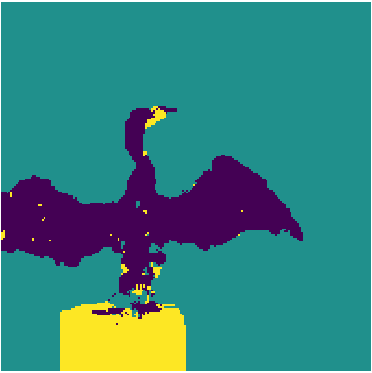
\includegraphics[width=0.6\textwidth]{imagenes/segmentacionlab}
\caption{Resultado de realizar la segmentación K-medias sobre Lab.}
\label{segmentacionlab}
\end{figure}

En el cuarto apartado de la práctica se trata la caracterización por textura como alternativa al color. Los filtros de textura se relacionan todos con características estadísticas como la entropía, la desviación estándar o el rango. Se escogen dos de estas características para realizar la segmentación con K-medias, en este caso, la entropía y la desviación estándar. En la Figura \ref{segmentacionse} se puede ver que los resultados no son buenos ya que segmenta los bordes del cormorán diferente del resto del cuerpo.\\
\begin{figure}[h]
\centering
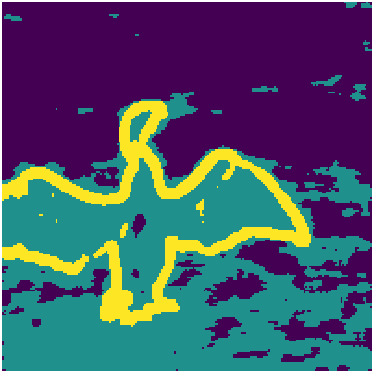
\includegraphics[width=0.6\textwidth]{imagenes/segmentacionse}
\caption{Resultado de realizar la segmentación K-medias sobre componentes de textura caracterizados por la desviación típica y la entropía.}
\label{segmentacionse}
\end{figure}

Por último, se prueba a usar varias características de distinta naturaleza, en este caso color y textura. Se cogen las características a y b del espacio de color Lab y la entropía, se estandarizan las 3 características y se aplica K-medias. La imagen resultante queda sobresegmentada con pequeñas regiones dentro del cuerpo del ave mal etiquetadas. Para solucionar esto se sugiere aplicar un filtro de media sobre las características de color. El resultado de la segmentación mejora como se puede apreciar en la Figura \ref{segmentacionabe}.\\ 

\begin{figure}[h]
\centering
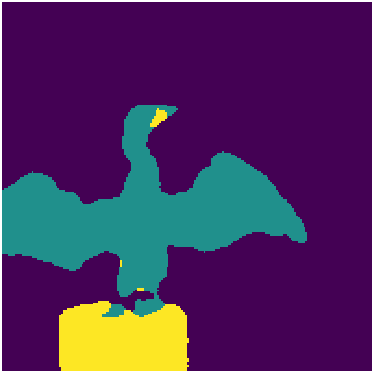
\includegraphics[width=0.6\textwidth]{imagenes/segmentacionabe}
\caption{Resultado de realizar la segmentación K-medias sobre componentes de color y textura.}
\label{segmentacionabe}
\end{figure}

El pico del pájaro nunca quedará segmentado como parte del ave en este ejercicio, ya que en cuestión de color el pico se parece más al tronco sobre el que se posa el ave que al cuerpo.\\


\subsection{Comparativa Matlab vs Python}

El primer apartado de la práctica se ha mantenido idéntico, ya que no requiere nada más que la función de representación del histograma.\\

En el siguiente apartado, lo primero que se pide es recolocar los datos de la imagen de modo que queden en una matriz con 3 columnas y tantas filas como píxeles tiene la imagen. Cada columna contiene los datos de una de las componentes de color RGB, esto nos sirve para la representación en forma de \emph{scatter plot}. Para convertir una matriz de dos dimensiones en un vector Numpy tiene la función de \texttt{reshape}. \\

Para aplicar K-medias vamos a usar la clase \texttt{Kmeans} de la biblioteca Scikit-learn. Primero se inicializa la clase indicando el número de centroides. Después se llama a la función \texttt{fit\_predict} con nuestra matriz de datos como parámetro. Esta función es la que ejecuta el algoritmo, por defecto se realizan un máximo de 10 iteraciones. En el atributo \emph{cluster\_centers} se guarda la posición final de los centroides y en \emph{labels} la capa de etiquetas que es una matriz con la misma forma que la matriz de datos. El resultado de este apartado es idéntico al de Matlab. \\

Para representar la capa de etiquetas hay que realizar las transformaciones inversas a las del inicio del apartado. En la figura \ref{comprgb} se puede ver las capas de etiquetas obtenidas en Matlab y Python. \\

\begin{figure}[!tbp]
  \centering
  \subfloat[Matlab]{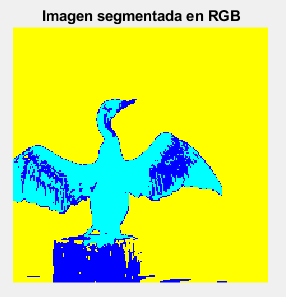
\includegraphics[width=0.4\textwidth]{imagenes/segmentacionrgbml}\label{fig:f1}}
  \hfill
  \subfloat[Python]{
\includegraphics[width=0.4\textwidth]{imagenes/segmentacionrgb}\label{fig:f2}}
  \caption{Comparativa de resultado en la capa de etiquetas}
  \label{comprgb}
\end{figure}

En el apartado sobre segmentación en el espacio de color Lab tanto en Matlab como en Python se usa una función específicamente programada para este ejercicio para pasar de RGB a Lab. En ambos lenguajes existe una función que hace esta transformación, la razón por la que no se usa es el tipo de transformación Lab que utilizan. Las normas que definen un espacio de color respecto a otro se han ido revisando y cambiando con el tiempo. La versión de Lab con la que se planteó esta práctica es la descrita en la norma de 1976\footnote{ISO 11664-4:2008(E)/ CIE S 014-4/E:2007 Colorimetry - Part 4: CIE 1976 L*a*b* Colour Space}, mientras que la función que convierte de RGB a Lab en Scikit-image usa la norma de 1999\footnote{IEC 61966-2-1:1999}.\\

 Para mantener la práctica tal y como se planteó se ha creado la función \texttt{RGB2LAB76} aunque también se ha hecho una versión de esta práctica con la función de Scikit-image. En la Figura \ref{normaslab} se puede ver la representación de las componentes a y b en las diferentes normas y en la Figura \ref{comparativalab} se muestra la diferencia en la segmentación con K-medias.\\

\begin{figure}[!tbp]
  \centering
  \subfloat[Norma de 1976.]{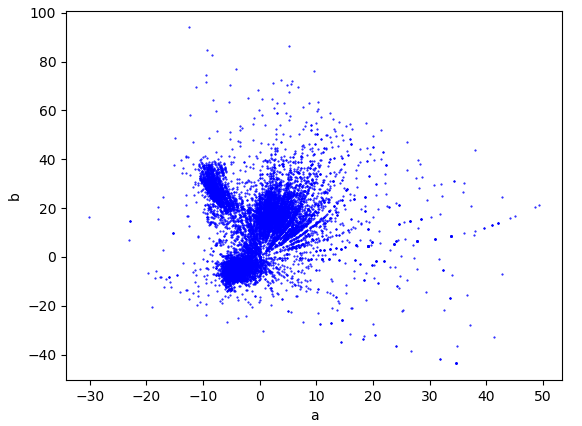
\includegraphics[width=0.4\textwidth]{imagenes/lab76}\label{fig:f1}}
  \hfill
  \subfloat[Norma de 1999]{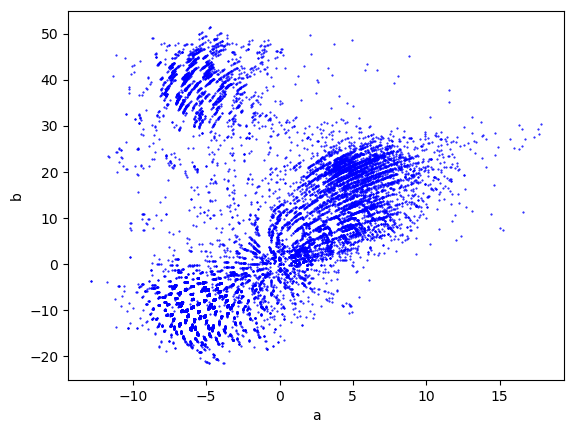
\includegraphics[width=0.4\textwidth]{imagenes/lab99}\label{fig:f2}}
  \caption{Diferencias entre las componentes a y b en las diferentes normas.}
  \label{normaslab}
\end{figure}

\begin{figure}[!tbp]
  \centering
  \subfloat[Norma de 1976.]{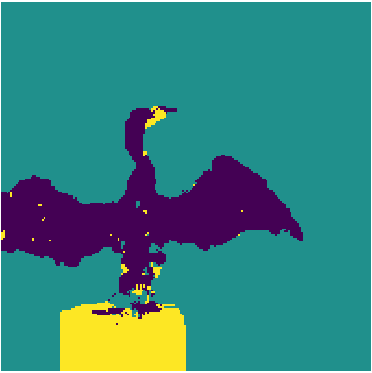
\includegraphics[width=0.4\textwidth]{imagenes/segmentacionlab}\label{fig:f1}}
  \hfill
  \subfloat[Norma de 1999]{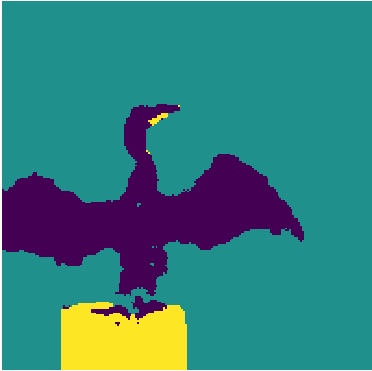
\includegraphics[width=0.4\textwidth]{imagenes/segmentacionlab99}\label{fig:f2}}
  \caption{Resultados de la segmentación con las diferentes normas de Lab.}
  \label{comparativalab}
\end{figure}

En este apartado se pide la normalización de las variables. La secuencia de código necesaria viene dada en el enunciado y esto se ha replicado en el cuadernillo de Jupyter modificando el código para funcionar en Python.\\

En el apartado de texturas, Matlab tiene funciones para realizar los diferentes filtros necesarios. En Python existe un equivalente del filtro de entropía con resultados idénticos. Los otros dos filtros no tienen equivalente en Python por lo que se han tenido que programar. Los resultados son muy similares, como se puede comprobar en la Figura \ref{texturas}.\\


\begin{figure}[!tbp]
  \centering
  \subfloat[Matlab]{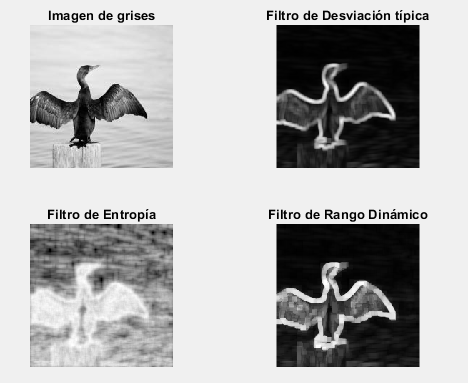
\includegraphics[width=0.5\textwidth]{imagenes/texturasml}\label{fig:f1}}
  \hfill
  \subfloat[Python]{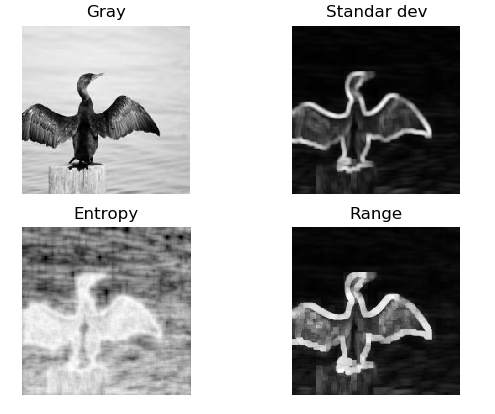
\includegraphics[width=0.5\textwidth]{imagenes/texturas}\label{fig:f2}}
  \caption{Comparativa filtros de textura en Matlab y Python.}
  \label{texturas}
\end{figure}

El último apartado utiliza herramientas ya empleadas en el resto de la práctica y un filtro de media explicado en la práctica 2.\\

\subsection{Desarrollo de funciones}

En este ejercicio se desarrollan 3 funciones nuevas:
\begin{itemize}

	\item \texttt{ RGB2Lab76}\footnote{\url{https://github.com/RoboticsLabURJC/2019-tfg-ana-cuevas/blob/master/PracticasTDI/P5/colorspacefunctions.py}}: Esta función realiza el cambio de espacio de color acorde a la norma de 1976. Primero se pasa de RGB a XYZ multiplicando cada componente por una serie de índices. Para pasar de XYZ a Lab se crean una serie de índices acotando los valores de cada componente de XYZ para sacar las coordenadas en el nuevo espacio de color. En la Figura \ref{colorspaces} se pueden ver los espacios de color RGb y Lab.
\begin{figure}[!tbp]
  \centering
  \subfloat[RGB]{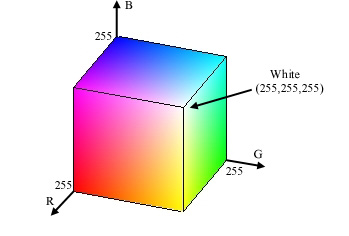
\includegraphics[width=0.5\textwidth]{imagenes/rgb}\label{fig:f1}}
  \hfill
  \subfloat[CIE Lab]{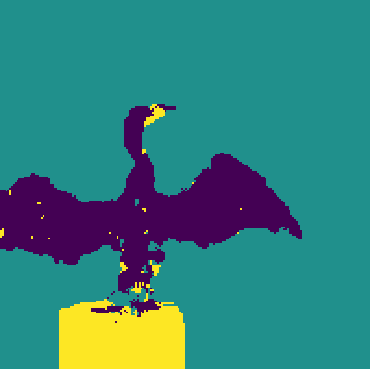
\includegraphics[width=0.5\textwidth]{imagenes/lab}\label{fig:f2}}
  \caption{Espacios de color RGB y CIE Lab.}
  \label{colorspaces}
\end{figure}

	\item \texttt{ stdfilt}: Esta función devuelve la imagen filtrada acorde a su variación estándar. Funciona de una manera similar a un filtro de media, con una máscara por defecto de tamaño 3x3 pero, en lugar de hacer la media con los píxeles debajo de la máscara, calcula su desviación estándar.

	\item \texttt{rangefilt}: Un filtro de rango devuelve el rango de valores bajo una máscara, que es la diferencia entre el máximo valor y el mínimo. Para programar este filtro se han empleado herramientas morfológicas. Se usa la operación de erosión como un filtro para conseguir el mínimo bajo el elemento estructural y la dilatación como un filtro de máximo. La resta de los resultados de la dilatación y erosión devuelve el rango.\\
\end{itemize}

Las 3 funciones de textura se encuentran en el mismo documento: 'texturefilters.py\footnote{\url{https://github.com/RoboticsLabURJC/2019-tfg-ana-cuevas/blob/master/PracticasTDI/P5/texturefilters.py}}

\section{Práctica 6: Morfología binaria}
\subsection{Teoría tratada}

Esta práctica\footnote{\url{https://github.com/RoboticsLabURJC/2019-tfg-ana-cuevas/blob/master/PracticasTDI/P6/6_Morphology.ipynb}} se centra en el uso de la morfología matemática para la segmentación de una imagen. Los operadores morfológicos son una serie de operadores no lineales relacionados con la forma de los objetos en la imagen. Como en las dos prácticas anteriores se va a usar la segmentación de una imagen en concreto para demostrar el funcionamiento de estos operadores. En este caso la imagen es de un circuito impreso, el objetivo es segmentar los 7 chips que se pueden ver en la Figura \ref{placa}\\

\begin{figure}[h]
\centering
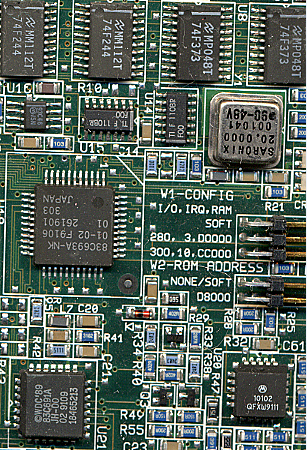
\includegraphics[width=0.6\textwidth]{imagenes/placa}
\caption{Imagen utilizada en la Práctica 6.}
\label{placa}
\end{figure}

Al igual que en la práctica anterior, lo primero que se va a hacer es decidir en qué espacio de color es más cómodo trabajar para esta segmentación. Tras probar en RGB se decide usar HSI, que es un espacio de color que define tono, saturación e intensidad. Mientras que en RGB las tres componentes se veían igual debido a la prominencia de tonos grises en la imagen, en HSI podemos apreciar una gran diferencia entre componentes. En la componente S se ven claramente diferenciados los chips, así que es la que se escoge para continuar el proceso de segmentación.\\

A continuación, se usa la umbralización para trabajar sobre una imagen binaria. Tras este proceso queda algún pixel blanco dentro de los chips que nos interesa eliminar. Se usa un filtro de mediana para homogeneizar la superficie de los chips.\\

En el siguiente apartado, se empiezan a usar operadores morfológicos. Contamos con 4 operadores morfológicos diferentes: erosión, dilatación, apertura y cierre. Para aplicar un operador morfológico se debe usar un elemento estructural. Los operadores morfológicos modifican los píxeles debajo del elemento estructural. La dilatación, por ejemplo, se queda con el máximo valor bajo el elemento estructural, la erosión el mínimo. La apertura y el cierre son elementos compuestos. La apertura es realizar una dilatación tras una erosión y el cierre lo opuesto según se muestra en la Figura \ref{erosion}\\

\begin{figure}[h]
\centering
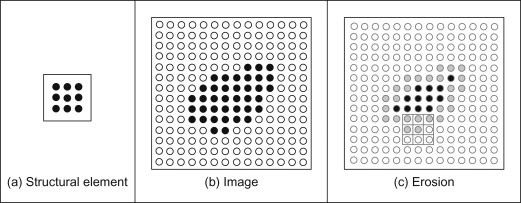
\includegraphics[width=0.8\textwidth]{imagenes/erosion}
\caption{Ejemplo del funcionamiento del operador morfológico erosión.}
\label{erosion}
\end{figure}

Para demostrar el efecto de cada uno de estos operadores morfológicos, en la práctica se pide que se usen todos sobre la imagen binaria a segmentar probando a cambiar el tamaño del elemento estructural. El objetivo es decidir qué operador morfológico es más apropiado para esta situación y terminar el apartado con una imagen en la que solamente están diferenciados los chips como la de la Figura \ref{closing} que es el resultado de aplicar cierre sobre la imagen.\\

\begin{figure}[h]
\centering

\includegraphics[width=0.6\textwidth]{imagenes/Closing}
\caption{Resultado de aplicar cierre sobre la imagen.}
\label{closing} 
\end{figure}

Para realizar la segmentación se invierte la imagen de forma que queden los chips en primer plano. Se segmenta la imagen usando segmentación binaria.\\

La práctica tiene dos apartados más: el primero pide que se use la excentricidad de las etiquetas para separar los chips cuadrados de los rectangulares, esto se hace de la misma manera que en la práctica 4 cuando se discriminaron etiquetas por su área. El segundo y último apartado pide que se usen operadores morfológicos para conseguir los bordes de los chips. Esto se consigue restando el resultado de la dilatación (que expande objetos) menos la erosión (que reduce el tamaño).\\

\subsection{Comparativa Matlab vs Python}

A la hora de desarrollar el cuadernillo, la primera complicación se encuentra al pasar la imagen de RGB a HSI. En la práctica original, esta función viene dada con el enunciado. En OpenCV tampoco existe esta función por lo que  se tiene que desarrollar de cero. El resultado es idéntico al de Matlab.\\

OpenCV tiene una función con un amplio rango de opciones para operadores morfológicos.  Para la erosión y la apertura se usan funciones dedicadas (\texttt{erode} y \texttt{dilate}), mientras que para la apertura, cierre y otros operadores se usa la misma funcion (\texttt{morphologyEx}) indicando la operación a realizar con un parámetro. Para el elemento estructural se usa una matriz de Numpy.\\

Para diferenciar los chips cuadrados de los rectangulares se mantiene igual, ya que la función \texttt{regionprops} de Scikit-omage también tiene la característica de excentricidad.\\

En el último apartado, cuyo objetivo es la detección de bordes, se usa un elemento estructural circular. Matlab  tiene una función para crear elementos  estructurantes de diferentes tamaños. OpenCV tiene una equivalente. El operador morfológico para detección de bordes se llama gradiente y la función \texttt{morphologyEx} permite aplicarlo directamente pero, ya que la práctica original pide que se razone cómo se obtendrían los bordes, se ha decidido mantener el proceso tal y como estaba. Al final del cuadernillo se menciona la existencia de esta función como información adicional.

\subsection{Desarrollo de funciones}

Este ejercicio ha requerido el desarrollo de una función para cambiar del espacio de color RGB a HSI\footnote{\url{https://github.com/RoboticsLabURJC/2019-tfg-ana-cuevas/blob/master/PracticasTDI/P6/RGB2HSI.py}}. Solo tiene un parámetro de entrada y uno de salida: la propia imagen en \texttt{uint8}. No es una función demasiado compleja ya que solamente aplica las fórmulas matemáticas necesarias para esta transformación, como se muestra en la Figura \ref{rgb2hsi}.

\begin{figure}[h]
\centering
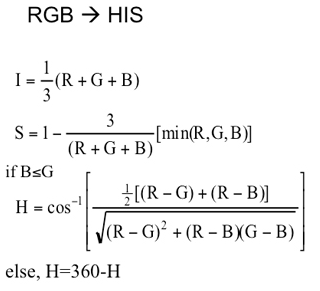
\includegraphics[width=0.6\textwidth]{imagenes/rgb2hsi}
\caption{Fórmulas para pasar de RGB a HSI.}
\label{rgb2hsi} 
\end{figure}

\section{Práctica 7: Segmentación con \emph{Watershed}}
\subsection{Teoría tratada}

Esta práctica\footnote{\url{https://github.com/RoboticsLabURJC/2019-tfg-ana-cuevas/blob/master/PracticasTDI/P7/7_Watershed.ipynb}} trata el método de segmentación por \emph{Watershed} con marcadores para contar el número de células enteras que hay en una imagen.\emph{ Watershed} es un algoritmo de segmentación basado en morfología matemática que trata la imagen como una serie de desniveles topográficos que forman picos y valles (Figura \ref{watershed}) que se van inundando. Se cogen las depresiones de intensidad como marcadores de los que crece el agua (la etiqueta). El proceso de inundación continúa hasta que toda la imagen está ``inundada'' y donde se toca el agua de diferentes regiones se forman las líneas de  \emph{Watershed} que limitan las regiones.\\

\begin{figure}[h]
\centering
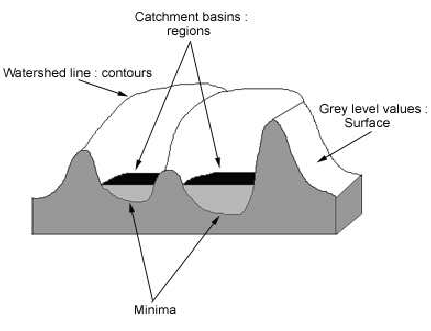
\includegraphics[width=0.6\textwidth]{imagenes/valles}
\caption{Ejemplo de \emph{Watershed}.}
\label{watershed} 
\end{figure}

Para que \emph{Watershed} funcione de la manera deseada es necesario extraer los marcadores que indicarán los valles. Primero se extraen los marcadores internos, para ello se trata la imagen en escala de grises con un filtro secuencial alternado que se utiliza para suavizar la imagen. Los filtros secuenciales alternados consisten en realizar de forma secuencial una serie de operaciones morfológicas con diferente elemento estructural. En este caso, se alterna entre apertura y cierre con elementos estructurales con forma de disco de radios 1, 2 y 3.\\

A continuación, se va a usar reconstrucción, que es una operación morfológica que toma una imagen (\emph{marker}) y la dilata repetidamente hasta que su forma coincide con otra imagen (máscara). Para crear el marcador aplicamos erosión sobre el negativo y usamos el propio negativo como máscara.\\ 

El siguiente paso es extraer los mínimos regionales. Un mínimo regional es una región (conjunto de píxeles conexos del mismo nivel) cuyo nivel es inferior al de todos los píxeles que la rodean. Esto devuelve una imagen binaria con más regiones que células en la imagen. Para reducir el número de regiones se usan 2 procesos diferentes:\\

Primero se limpian los bordes, no nos interesan células que no estén enteras, ya que, podrían aparecer en la siguiente imagen de microscopio y ser contadas dos veces.\\

El segundo proceso consiste en comparar la posición de nuestras regiones con la posición de los núcleos de las celdas en la imagen original basándonos en que los núcleos aparecen en un color más oscuro. Se eliminan todas las regiones cuya posición coincida con un pixel demasiado claro en la imagen original para ser un núcleo.El resultado de estos dos procesos se puede ver en la Figura \ref{procesos}

\begin{figure}[!tbp]
  \centering
  \subfloat[Máximos regionales.]{
\includegraphics[width=0.4\textwidth]{imagenes/Imaxreg}\label{fig:f1}}
  \hfill
  \subfloat[Máximos regionales procesados.]{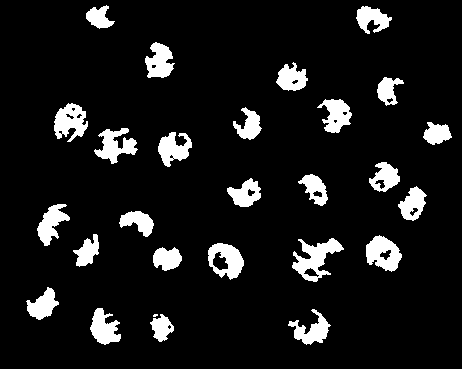
\includegraphics[width=0.4\textwidth]{imagenes/Imaxreg3}\label{fig:f2}}
  \caption{Proceso para conseguir los marcadores internos.}
  \label{procesos}
\end{figure}

Con eso ya tendríamos los marcadores internos. Para conseguir los marcadores externos (o de fondo) dilatamos la imagen de los marcadores internos para salir de la célula y hacemos una transformada de distancia que es una operación que devuelve una imagen en escala de grises donde el valor de cada píxel corresponde a la distancia a la que se encuentra de un píxel de primer plano. Los píxeles de primer plano en la transformada de distancia tienen valor 0.\\

Sobre la imagen de la transformada de distancia aplicamos  \emph{Watershed}. Los bordes que se forman entre regiones marcan los marcadores externos, siendo los puntos más alejados del nucleo de cada célula.\\

A continuación se crea una imagen que combina los marcadores internos y externos (Figura \ref{marcadores}). \\

\begin{figure}[h]
\centering
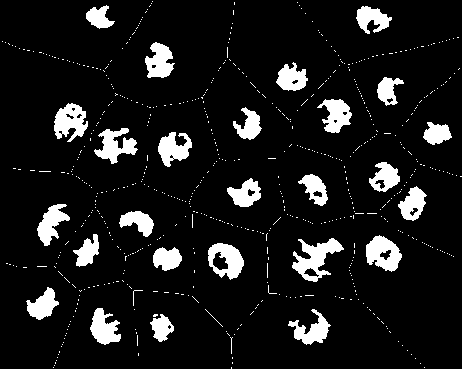
\includegraphics[width=0.6\textwidth]{imagenes/marcadores}
\caption{Marcadores internos y externos.}
\label{marcadores} 
\end{figure}

Para conseguir los bordes reales de las células se vuelve a aplicar  \emph{Watershed}, pero esta vez usando marcadores. Como imagen de referencia, en lugar de la transformada de distancia, se usa el gradiente de la imagen reconstruido de forma que nuestros marcadores queden como los únicos mínimos regionales y que los bordes de las células sean los puntos de mayor intensidad de la imagen mientras que el fondo y los núcleos, al tener menos variación, tienen menor intensidad. En la Figura \ref{finalwatershed} se puede ver el resultado final de esta práctica.\\

\begin{figure}[h]
\centering
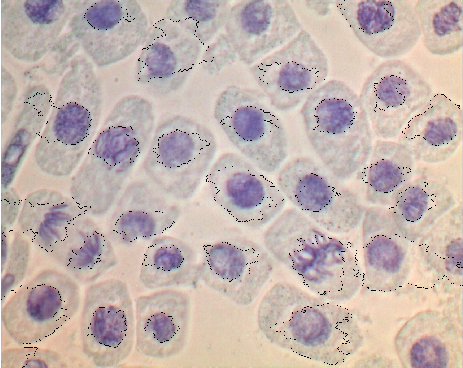
\includegraphics[width=0.6\textwidth]{imagenes/finalwatershed}
\caption{Resultado de la práctica de \textbf{Watershed}.}
\label{finalwatershed} 
\end{figure}



\subsection{Comparativa Matlab vs Python}

La primera diferencia en esta práctica entre Matlab y Python es la imagen empleada. La imagen original fue sacada de un artículo que no se ha podido localizar y se desconoce su licencia de copyright. Se ha encontrado otra imagen también de células muy cercanas las unas a las otras, en este caso de cebolla.\\

El primer apartado se mantiene igual en cuanto a funciones empleadas pero los resultados no son los mismos. Esto se debe al tipo de \emph{padding} que usan las funciones de apertura y cierre en Matlab y Python y que no se permiten modificar. En el caso de Matlab cuando hace erosión usa \emph{padding} 1, mientras que para dilatar usa ceros. En la función de OpenCV no indica el \emph{padding} que usa pero, por los resultados, parece que usan \emph{mirror padding}. Esto crea una diferencia en los valores cercanos al borde que en este caso no genera problemas pero que se tiene que tener en cuenta para otros casos.\\

Debido al cambio de imagen algunos de los valores empleados como elemento estructural se han tenido que cambiar, es el caso del elemento estructural usado para la erosión antes de la reconstrucción. Para la reconstrucción se encuentra una función en Scikit-image que funciona exactamente igual al equivalente en Matlab. \texttt{Imreconstruct} en los dos casos recibe una imagen de máscara y una de marcadores.\\

\texttt{ImregionalMax} es una función de Matlab que devuelve los máximos regionales de una imagen. En Python no existe ninguna función equivalente por lo que se ha tenido que programar. La nueva función devuelve exactamente el mismo resultado que la de Matlab.\\

A continuación, se eliminan los marcadores que corresponden a las células del borde de la imagen que no están completas. En Matlab se usa la función \texttt{imclearborder}. En Python no hay versión en ninguna librería oficial, pero se ha encontrado una versión en Github subida por el usuario hatamiarash7\footnote{\url{https://github.com/hatamiarash7/Python-Projects/blob/master/OpenCV/}} que cumple la misma función.\\

Lo siguiente es eliminar los marcadores que no coincidan con un núcleo en la imagen original. En Matlab se usa la función\texttt{ regionprops} con el atributo \emph{mean intensity}, \texttt{regionprops} en Scipy-image tiene el mismo atributo con el mismo funcionamiento.\\

Para obtener los marcadores externos se usa la función de dilatar ya mencionada en la práctica anterior y la transformada de distancia, para realizarla Matlab tiene la función \texttt{bwdist} mientras que OpenCV tiene \texttt{distancetransform}. La principal diferencia entre estas dos funciones es que trabajan al revés: la de Matlab devuelve la distancia al punto de primer plano más cercano, mientras que la versión OpenCV devuelve la distancia a 0. Esto se resuelve pasando el negativo de los marcadores a la función en el cuadernillo de Jupyter.\\

A continuación, se aplica \emph{Watershed} sobre esta imagen. En Matlab la función de \texttt{Watershed} recibe como argumento la imagen a segmentar. En Python tenemos dos opciones aunque ninguna funciona exactamente igual que la de Matlab.\\

La primera que se prueba es la versión de OpenCV que se descarta inmediatamente, ya que requiere una imagen RGB como primer argumento y la imagen que queremos pasar nosotros es en escala de grises.\\

La segunda opción es la de Scikit-image, también llamada \texttt{watershed}. Esta sí que permite imágenes en escala de grises. La principal diferencia con Matlab es que como segundo argumento pide una imagen binaria de marcadores y si no viene especificada como marcadores se eligen los mínimos locales de la imagen. En la versión de Matlab se cogen los mínimos regionales. En este primer uso de \emph{Watershed} la diferencia no es relevante ya que coinciden los mínimos.\\

 Otra diferencia, ya menor, es que la versión de Matlab automáticamente devuelve las fronteras señaladas en la imagen con un 0 de etiqueta, mientras que en la versión de Scikit-image se tiene que especificar que se requiere etiqueta para las líneas de \emph{Watershed}.\\

Con esto ya tenemos los marcadores, tanto internos como externos. A continuación se usa un filtro paso alto para sacar el gradiente del mismo modo que se hizo en la práctica 2. Y se vuelve a aplicar  \emph{Watershed}, esta vez la diferencia entre los mínimos sí que es relevante así que, en la versión de la práctica en Python, a la función de \texttt{watershed} además de pasarle el gradiente con marcadores como segundo argumento se pasa la imagen binaria de marcadores.\\


\subsection{Desarrollo de funciones}

Para esta práctica se ha tenido que desarrollar la función \texttt{imregionalmax}\footnote{\url{https://github.com/RoboticsLabURJC/2019-tfg-ana-cuevas/blob/master/PracticasTDI/P7/imregionalmax.py}}. Esta función toma la imagen de la que se quiere conseguir los máximos regionales y se le resta 1. A continuación, se hace reconstrucción con la imagen original como máscara y la imagen a la que hemos restado 1 de marcador sobre el que se va realizando la dilatación repetida de la reconstrucción. Esto genera una imagen cuya única diferencia con la original son las regiones de máximos. Si restamos el resultado de la reconstrucción a la imagen original obtenemos una imagen en la que los únicos valores diferentes de cero son los máximos regionales. Esta imagen se pasa a binario y es lo que devuelve la función \texttt{imregionalmax}.


\section{Práctica 8: Video y estimación de movimiento}
\subsection{Teoría tratada}

Esta práctica\footnote{\url{https://github.com/RoboticsLabURJC/2019-tfg-ana-cuevas/blob/master/PracticasTDI/P8/P8_Video.ipynb}} es la primera práctica de video. Tiene dos partes muy marcadas.\\

La primera es una introducción a las herramientas de video. Se muestra cómo leer un video, visualizar los fotogramas, en qué consiste el \emph{frame rate} y cómo afecta a la reproducción de video. Se pide que se modifiquen un par de fotogramas con transformaciones como filtros y pasar a negativo para comprobar qué transformación es más perceptible.\\

La segunda se centra en demostrar la estimación de movimiento basada en bloques, específicamente 3 algoritmos: EBMA, HBMA y correlación de fase.\\

La estimación de movimiento basada en bloques se utiliza para codificación de vídeo. Estos algoritmos se dividen en dos grupos: algoritmos en el dominio del tiempo (EBMA y HBMA) y algoritmos en el dominio de la frecuencia (correlación de fase).\\

EBMA (\emph{exhaustive block-matching algorithm}) consiste en una búsqueda exhaustiva por bloques comparando en el fotograma actual el bloque más similar al del bloque de referencia. Es el menos eficiente de los algoritmos, pero el más preciso.\\

HBMA(\emph{hierarchical block-matching algorithm}) funciona de una manera similar a EBMA, pero primero busca cambios en bloques más grandes y una vez localizadas las áreas de cambio reduce el tamaño de los bloques a comparar en esta nueva área. Esto hace que sea un algoritmo más eficiente.\\

El último algoritmo que se demuestra en esta práctica es el de correlación de fase, que trabaja en frecuencia comparando las fases de los dos fotogramas.\\

Para comparar el funcionamiento de los algoritmos se calcula el MSE (\emph{mean stimation error}) de cada uno.\\

\subsection{Comparativa Matlab vs Python}

En la primera mitad de esta práctica lo que genera la mayor diferencia es la forma de tratar el video entre los dos lenguajes de programación. Cuando lees un video en Matlab, usando la función \texttt{videoreader}, esta devuelve una variable que contiene todos los fotogramas del video y otra información como el número de fotogramas, el \emph{framerate} y el tamaño del video. Al llamar a la función \texttt{VideoCapture} de OpenCV lo que se crea es un objeto de la clase VideoCapture con una serie de métodos que en algunos casos devuelven la misma información que contiene la variable de video de Matlab.\\

En Matlab, lo primero que se pide es leer el video e inspeccionar la variable que se crea en el \emph{workspace}. Para simular esto en Python se crea una instancia de la clase \texttt{VideoCapture} y se van guardando los fotogramas en un array usando la función \texttt{read()}. \texttt{VideoCapture} en OpenCV permite capturar directamente video de la cámara que esté conectada al ordenador pero, en este caso, se usa el video \texttt{'shopping\_center.mpg'} que es el mismo que se usa en la versión de la práctica en Matlab.\\

A continuación, en la práctica de Matlab se piden una serie de características del video que se pueden obtener de la variable. En Python, se puede averiguar llamando al método \texttt{get()} de la clase \texttt{VideoReader}. Esto nos permite saber el ancho y alto de cada fotograma y el \emph{framerate}. Conseguir el número de fotogramas es algo más complejo, ya que el contador de fotogramas del método \emph{get()} es bastante inexacto y tiende a fallar. La mejor forma de saber el número de fotogramas es mirando la longitud del array guardado en el apartado anterior.\\

Posteriormente, se inspecciona el primer fotograma. En esto no hay diferencia con cómo se representan imágenes en prácticas anteriores.\\

A la hora de reproducir el video se puede usar \texttt{imshow} de OpenCV en un bucle pero esto abre una nueva ventana. Se intenta el mismo método con Matplotlib pero la reproducción no es fluida. Para solucionar esto, se usa una nueva librería: Bokeh. Es una librería de representación de gráficos que permite embeberlos en el cuadernillo. La reproducción de video queda fluida pero esta librería lee las imágenes con el eje girado y en el espacio de color RGBA por lo que hay que transformar cada fotograma antes de reproducirlo. Se usa un buble while y la función \texttt{time.sleep()} de Python para que se pinte un nuevo fotograma cada 1/25 segundo, lo indicado por el \emph{framerate} del video.\\

El siguiente punto del ejercicio pide reproducir el video con un \emph{framerate} distinto.\\

En la parte de estimación de movimiento, en Matlab, se utilizan 3 funciones programadas para la asignatura. En Python se hace lo mismo consiguiendo los mismos resultados. \\

En este apartado se pide usar el algoritmo EBMA con 3 tamaños diferentes de bloque (8, 16 y 32), representar el fotograma estimado, el mapa vectorial que devuelve la función y calcular el MSE para cada una de las 3 instancias. La figura \ref{ebma32} muestra el fotograma estimado en Matlab y en Python con un tamaño de bloque de 32.\\

\begin{figure}[!tbp]
  \centering
  \subfloat[Matlab]{
\includegraphics[width=0.4\textwidth]{imagenes/ebma32ml}\label{fig:f1}}
  \hfill
  \subfloat[Python]{\includegraphics[width=0.4\textwidth]{imagenes/ebma32py}\label{fig:f2}}
  \caption{Comparativa de resultados EBMA con bloque 32.}
  \label{ebma32}
\end{figure}
A continuación se pide ejecutar HBMA con un bloque de tamaño 16 y 3 niveles.\\

Por último, ejecutar la función \texttt{PhaseCorrelation} que, automáticamente, representa el fotograma estimado, el mapa vectorial y devuelve el MSE.\\

Las diferencias en este apartado vienen a la hora de representar los vectores de movimiento. La función \texttt{quiver} de Matplotlib representa mapas vectoriales pero, a no ser que se le indique de otro modo, el tamaño de las flechas varía para que la representación quede más visualmente interesante. En la Figura \ref{arrow} se puede ver una comparación de la representación  de los vectores de movimiento del algoritmo EBMA con bloques de tamaño 8 en Matlab, en Matplotlib con los valores por defecto y en Matplotlib con los valores corregidos. Los vectores utilizados son exactamente iguales.\\

\begin{figure}[!tbp]
  \centering
  \subfloat[Matlab]{\includegraphics[width=0.3\textwidth]{imagenes/arrowml}\label{fig:f1}}
  \hfill
  \subfloat[Python sin modificar]{\includegraphics[width=0.3\textwidth]{imagenes/arrowpymala}\label{fig:f2}}
  \hfill
  \subfloat[Python mejorado]{\includegraphics[width=0.3\textwidth]{imagenes/arrowpybuena}\label{fig:f3}}
  \caption{Diferencias en el mapa de vectores de movimiento.}
  \label{arrow}
\end{figure}
\subsection{Desarrollo de funciones}

En esta práctica se han desarrollado 3 funciones, los algoritmos de estimación de movimiento. Los tres se encuantran en el mismo documento: 'motionalgorithms.py'\footnote{\url{https://github.com/RoboticsLabURJC/2019-tfg-ana-cuevas/blob/master/PracticasTDI/P8/motionalgorithms.py}}\\

\begin{itemize}
	\item \textbf{EBMA}: Esta función recibe 3 atributos: el fotograma de referencia (\emph{anchor frame}), el fotograma actual (\emph{target frame}) y el tamaño de bloque que se va a usar. La función empieza declarando variables como el ancho y alto de cada fotograma y los arrays que van a formar el mapa de vectores de movimiento.\\
 
A continuación, se itera por la imagen de referencia en saltos del tamaño del bloque, se define el bloque dentro del fotograma de referencia. Para buscar movimiento se va desplazando el bloque de referencia en diferentes posiciones sobre el fotograma actual buscando el mayor parecido en un número limitado de posiciones. Una vez encontrado el bloque más parecido se guarda en una matriz del mismo tamaño que los fotogramas. Esta matriz será el fotograma estimado. Se guarda en el array de origen la posición del bloque de referencia y en el array de destino la posición en el nuevo fotograma. Esto se repite hasta que se ha iterado por toda la imagen.\\

	\item \textbf{HBMA}: Este algoritmo es muy parecido al anterior pero para mejorar el rendimiento se añaden unos pasos previos. La idea es primero usar bloques más grandes para descartar las áreas en las que no hay cambios. Para estos bloques grandes se crea una nueva imagen de la mitad de tamaño que la original y manteniendo el tamaño de bloque original. Se recorre esta imagen más pequeña y se guarda en un array la posición de las áreas que han cambiado.\\

A continuación, se hace EBMA sobre la imagen original con el tamaño de bloque pedido (16 en este caso) pero sólo en las áreas marcadas en el paso anterior. Esto quiere decir que en lugar de recorrer la imagen original entera, como se hacía en la función anterior, sólo se recorren secciones específicas.\\

El tercer nivel funciona igual que el anterior: en las áreas de cambio detectadas en el paso anterior se hace EBMA sobre la imagen ampliada. Esto crea la sensación de que se ha usado un bloque de la mitad de tamaño esto hace que no se cambien más píxeles de los estrictamente necesarios.\\

	\item \textbf{PhaseCorrelation}: Esta función también calcula un fotograma estimado a partir de dos fotogramas diviéndolos en bloques, la diferencia con las dos anteriores es que, en este caso, se trabaja en frecuencia. Primero se define una ventana con forma de campana que se va a usar para suavizar los bordes del bloque. A continuación se va dividiendo la imagen en bloques y haciendo la transformada de Fourier de esos bloques.  Se calcula la coherencia entre el bloque actual y el bloque de referencia multiplicando el bloque actual por el conjugado del bloque de referencia y normalizando el resultado. Obtenemos la correlación de los dos bloques haciendo la transformada inversa del resultado de la operación anterior. A continuación se localizan los máximos que indican dónde se encuentra la mayor diferencia entre los bloques. Para terminar se sustituyen los valores creando una nueva matriz que será el fotograma estimado.
\end{itemize}

\section{Práctica 9: Filtrado en video}
\subsection{Teoría tratada}

La última práctica\footnote{\url{https://github.com/RoboticsLabURJC/2019-tfg-ana-cuevas/blob/master/PracticasTDI/P9/9_Videorestoration.ipynb}} de la asignatura trata el uso de filtros en video.\\

La práctica se estructura de una forma muy similar a la práctica 2. Se empieza contaminando el video con ruido Gaussiano y sal y pimienta para, a continuación, filtrar el video y comprobar los efectos de los filtros temporales. En la figura \ref{ruidovideo} se puede ver el fotograma original, el fotograma contaminado con ruido gaussiano y con ruido sal y pimienta.\\
\begin{figure}[h]
\centering
\includegraphics[width=1.0\textwidth]{imagenes/ruidovideo}
\caption{Un fotograma de video contaminado con dos tipos de ruido.}
\label{ruidovideo} 
\end{figure}

Se van a usar dos filtros temporales diferentes. Un filtro temporal es un filtro que en lugar de usar una máscara que coge píxeles del mismo fotograma cercanos al pixel que se está filtrando coge los píxeles en la misma posición de diferentes fotogramas.\\

El primero de los filtros que se usa es un filtro temporal de media que, como indica su nombre, hace la media  entre el número de fotogramas indicado para filtrar. Al analizar el video resultante de estos filtros se comprueba que los primeros fotogramas no quedan filtrados; esto se debe a que si, por ejemplo, estamos filtrando con 5 fotogramas, dos anteriores al fotograma actual y dos posteriores no se puede empezar a filtrar hasta el tercer fotograma.\\

El segundo filtro que usa es un filtro temporal de mediana que calcula la mediana de los fotogramas que se estén usando. La peculiaridad en esta práctica es que no se da una función para realizar este filtro si no que se pide que se modifique la función usada para el filtro de media.\\

\subsection{Comparativa Matlab vs Python}

La primera diferencia entre la versión de Matlab y Python de esta práctica es el video usado. Se ha escogido un video sin copyright de una librería que almacena videos para uso didáctico.\\

Al igual que pasaba en la práctica 2 no existe una función para añadir ruido en Python, de hecho en Matlab, tampoco existe una función para añadir ruido a videos. Se crea la función \texttt{addnoise} para contaminar una secuencia de video RGB. Los resultados son los mismos que en Matlab.\\

Ni en Python ni en Matlab existen funciones para aplicar filtros temporales por lo que se tiene que programar \texttt{tempNoiseFilter} para realizar un filtro de media temporal.\\ 

Tanto la función \texttt{addnoise} como \texttt{tempNoiseFilter} crean nuevos videos que quedan guardados en la misma carpeta de la práctica como se puede ver en la Figura \ref{carpetaP9}

\begin{figure}[h]
\centering
\includegraphics[width=0.8\textwidth]{imagenes/carpetaP9}
\caption{Contenido de la carpeta de la práctica 9 tras ejecutar addnoise y TempNoiseFilter.}
\label{carpetaP9} 
\end{figure}

\subsection{Desarrollo de funciones}

Esta práctica usa dos funciones principales: \texttt{addnoise} y \texttt{tempNoiseFilter}. Las dos guardades en el documento 'videofunctions.py'\footnote{\url{https://github.com/RoboticsLabURJC/2019-tfg-ana-cuevas/blob/master/PracticasTDI/P9/videofunctions.py}}\\

La función \texttt{addnoise} recibe como argumentos: el nombre del video a contaminar, el nombre que se le va a dar al video contaminado, el tipo de ruido y un array con los fotogramas a contaminar. En el caso de que el array esté vacío se contaminan todos los fotogramas. Esta función se sirve de varias funciones más pequeñas. Primero se usa \texttt{getfotogramas} que recibe el nombre del video y devuelve un array con todos los fotogramas. Tras una serie de comprobaciones (como que el array de fotogramas no esté vacío y el número de fotogramas a contaminar) se itera sobre cada fotograma llamando a la función \texttt{plusnoise} con el fotograma y el tipo de ruido y esta llama a la función \texttt{imnoise} usada en la práctica 2. La función \texttt{plusnoise} devuelve una imagen contaminada que se guarda en un nuevo array que formará parte de la nueva estructura de video contaminado. En la Figura \ref{addnoise} se puede ver el código de esta función.\\

\begin{figure}[h]
\centering
\includegraphics[width=1.0\textwidth]{imagenes/addnoise}
\caption{Imagen del código de la función addnoise.}
\label{addnoise} 
\end{figure}

La otra función \texttt{tempNoiseFilter}, al igual que en \texttt{addnoise}, sus primeros argumentos son los nombres del video de entrada y de salida. El tercer argumento de la función es el número de fotogramas que se va a usar para calcular la media. Primero se lee el video usando \texttt{getfotogramas}. A continuación se itera por el array de fotogramas calculando la media entre el número de fotogramas establecido. Al igual que \texttt{addnoise} guarda un nuevo video con el nombre indicado en el segundo argumento.\\
\chapter{Conclusiones}
En este capítulo se exponen las conclusiones obtenidas tras completar las 9 prácticas propuestas por la asignatura y los posibles trabajos futuros que pueden surgir a partir de este trabajo de fin de grado. 

\section{Resultados}
El objetivo principal planteado en el apartado 2 se ha cumplido, se han creado versiones en Python de las 9 prácticas de la asignatura de Tratamiento Digital de la Imagen.\\

Se han ampliado los enunciados tal y como se propuso intentando mantenerlos claros y amenos de forma que sean lo más didácticos posible y se han traducido al inglés.\\

El código se mantiene bastante similar y cuando no es exacto se ha mantenido lo que se pretendía demostrar con la práctica.\\

Las prácticas que más similares han quedado a su equivalente en Matlab son:
\begin{itemize}
    \item La práctica 2 de filtros en el espacio que, la única modificación, fue la creación de las funciones de ruido.
    \item La práctica 3 de imágenes en frecuencia cuya mayor diferencia es meramente estética, las representaciones 3D de Matplotlib crean un efecto más cuadriculado que las de Matlab pero cumplen la misma función.
    \item La práctica 4 que obtiene exactamente el mismo resultado aunque en el apartado sobre la capa de etiquetas hay una pequeña diferencia en el tratamiento del fondo.
    \item Las prácticas 5 y 6 ambas de segmentación han quedado exactamente igual.\\
\end{itemize}

El resto de prácticas tienen todas alguna gran diferencia para la que se ha tenido que encontrar una solución que mantenga la intención del ejercicio:
\begin{itemize}
    \item La práctica 1 es la que tiene una mayor desviación de la original en un apartado concreto: las imágenes indexadas. No se pudo encontrar una función equivalente y la programada tenía un tiempo de ejecución demasiado alto, por lo que, en lugar de crear imágenes indexadas en la práctica se importan y así se puede ver en qué consisten en el cuadernillo. También se tuvieron que cambiar dos de las imágenes utilizadas.
    
    \item Todas las diferencias en la práctica 7 surgen de tener que cambiar la imagen utilizada. Al ser una imagen diferente se han tenido que ir modificando pasos importantes. 
   
    \item Las dos prácticas de vídeo (8 y 9) tienen la misma diferencia con la original: la estructura de la variable en la que se guardan los vídeos en Matlab no existe en Python por lo que se han tenido que sustituir varios puntos que en la práctica original consistían en mirar la variable por apartados con nuevas funciones.\\ 
\end{itemize}


En cuanto a que las prácticas sean multiplataforma se ha conseguido con el uso de herramientas como Pipnv.\\

Por último, a un nivel personal este trabajo me ha permitido expandir mi conocimiento sobre la asignatura y el campo de tratamiento de imagen, también el uso de Python en este campo. He descubierto cosas nuevas como Pipnv o las librerías especializadas de Scipy. \\

Además me ha ayudado a mejorar en otras áreas más amplias como la búsqueda de información o la redacción. Es muy importante redactar bien, de una manera que ayude a entender un concepto y no complicarlo más. Me ha ayudado mucho a valorar el trabajo de los traductores de campos técnicos al tener que redactar tanto en inglés como en español.

\section{Trabajos futuros}

En cuanto a trabajos futuros hay varias opciones ya abiertas.\\

Para empezar, se ha planteado un estudio comparativo con varios alumnos para la implementación de estas nuevas prácticas en la asignatura de Tratamiento Digital de la Imagen  en el que unos realizarían las prácticas en Matlab y otros en Python. Después se evaluaría si esta nueva versión de las prácticas supone una mejora en el desarrollo de la asignatura. Para que este estudio se pueda llevar a cabo se tendrían que modificar los enunciados para que sean lo más parecido posible a los de Matlab. Esto se debe a que no todos los alumnos cursando la asignatura en la URJC tienen la misma facilidad para entender inglés que español y que la ampliación de los enunciados podría suponer una ventaja para los alumnos del grupo realizando las prácticas nuevas.\\

Otra posibilidad se basa en crear la opción de una implementación web, usando la ``implementación mixta" propuesta por Carlos Awadallah en su trabajo de fin de master\footnote{\url{https://gsyc.urjc.es/jmplaza/students/tfm-academy-carlos_awadallah-2020.pdf}}. Esto permitiría ejecutar las prácticas con un navegador en un servidor remoto lo que ahorraría el paso de instalación de las prácticas.\\

Otros posibles trabajos futuros tienen que ver con algunas mejoras en el código. Por ejemplo, la función \textttt{RGB2ind} se podría programar en C e implementar en Python para mejorar la velocidad de ejecución que es la razón por la que se tuvo que descartar.\\

Otra opción sería crear un mejor reproductor de video que se pueda implementar directamente en el cuadernillo de Jupyter. Como se ha comentado en las dos prácticas de video la reproducción de video con Matplotlib va dando tirones y es muy incómoda, aunque Bokeh lo mejora un poco sigue basándose en ir representado los diferentes fotogramas sobre la misma figura con un bucle \texttt{while}. La idea sería crear una función que directamente representase video y tuviera opciones típicas como parar, moverte fotograma a fotograma, adelantar o retroceder.\\

Cabe también la opción de contribuir a una biblioteca oficial con las nuevas funciones creadas. Scikit-image permite a usuarios incorporar nuevas funciones a la biblioteca pero para eso se tendrían que depurar un poco más, ya que tienen que pasar por un extenso proceso de revisión.\\

Por último, expandir el número de prácticas y el tema hacia campos más específicos. Por ejemplo crear una nueva práctica que use conocimiento de las anteriores pero orientarla más hacia el campo de la robótica de forma que se puedan apreciar más los usos reales de este campo.\\

\nocite{*}

\begingroup
\raggedright
\sloppy
\printbibliography
\endgroup
\end{document}